
In this section, we present the results obtained from the multiple conducted experiments of the overlay protocol against state-of-the-art baselines. These experiments aimed at testing: (1) the cost of establishing/maintaining the overlay networks for each protocol; (2) testing the established networks' efficiency (according to latency); and (3) finally, testing DeMMons' message dissemination capabilities against that same set of baseline protocols. In this last test, the baseline membership protocols are paired with two distinct dissemination protocols to perform the message dissemination. We now begin by providing a brief discussion of the protocols and parameters used for conducting the experiments.

\subsection{Baselines and configuration parameters}

The chosen protocols to perform the overlay protocol network comparison were \textbf{Hyparview} \cite{Hyparview}, \textbf{X-Bot} \cite{x-bot}, \textbf{Cyclon} \cite{voulgaris2005Cyclon} and \textbf{T-Man} \cite{t-man}. We now provide a brief description of each (further discussion is provided in Section \ref{sec:topology_management}).

\textbf{Hyparview} is a protocol that builds a non-structured overlay network using a fixed-sized view materialized by active bidirectional TCP connections (these connections also serve as fault detectors). 

The second baseline protocol is \textbf{X-Bot} \cite{x-bot}, which is a protocol that essentially behaves similarly to Hyparview in terms of establishing the initial network structure but takes iterative steps to optimize the overlay network (according to a configurable heuristic). These steps are performed via gossip mechanisms to improve the nodes' active connections' costs. In X-Bot, nodes perform optimizations in such a way that maintains the in and out-degree established initially. 

The third implemented baseline protocol was \textbf{Cyclon} \cite{voulgaris2005Cyclon}, which is an overlay protocol that materializes a network composed of asymmetric links via periodic exchanges of node pointers with a configurable age. 

The last implemented baseline was \textbf{T-Man} \cite{t-man}, which is a protocol that iteratively builds on an existing set of nodes to build a new, more optimized set of nodes. These optimizations are performed iteratively by each node in the system such that a configurable cost function (defined a priori) gets minimized. In order to feed the initial node sample for T-man to optimize, we employed the Cyclon protocol, and consequently, the evaluation results for this protocol are labelled as ``Cyclon T-Man''. All of the described baseline protocols were, for comparativeness, implemented using the GO-Babel framework (described in Section \ref{sec:Node-Watcher}). As Go-Babel only provides unidirectional connections, protocols that require bidirectional connections, namely Hyparview, X-Bot and DeMMon, were enriched with added mechanisms to ensure that the bidirectional connections were established for each node contained in nodes' active views.

The utilized parameters for the different protocols were tuned to attempt to perform a fair comparison. These are displayed in table \ref{table:proto_test_params}, we now describe each of the columns. The first is called ``VSizeMax'', and represents the maximum size of the active view, which in most protocols was set to 5, except for Cyclon, where it was set to 7 as it is the only protocol without a secondary backup view. In the case of DeMMon, ``VSizeMax'' represents the maximum number of children per node. 

The second column, named ``VSizeMin'', corresponds to the minimum number of children for each node in DeMMon. The third parameter, titled ``PVSizeMax'', corresponds to the maximum size of the passive view, which is set to 25 for DeMMon, Hyparview and X-BOT, and set as 7 for the case of Cyclon T-Man. In the case of T-man, this parameter corresponds to the size of the Cyclon view (running to provide its initial view). The next parameter, labelled ``Shuffle'', corresponds to the periodicity of each protocols' shuffle mechanism. This parameter is set to 5 seconds for all protocols. Following, we have the ``PWRL'' parameter, which corresponds to the TTL of the random walks (for each protocol that has a random walk mechanism). The last-mentioned parameter is the ``$\delta$T'' parameter, which corresponds to the minimum latency improvement for both X-Bot to perform active view exchanges and for DeMMon to make opportunistic improvements. Some parameters such as timeouts and the duration of some periodic procedures were omitted, however, all timeouts, e.g. timeouts for dialling nodes, receiving message responses, among others, are set to 5 seconds. Furthermore, all periodic mechanisms are executed with a frequency lower than 15 seconds.

\begin{table} \label{table:proto_test_params}
    \caption{Membership evaluation: protocol configuration parameters}
    \scalebox{1}{
    \centering
    \resizebox{\textwidth}{!}{%
    \begin{tabular}{llllllllllll}
                & VSizeMax & VSizeMin & PVSizeMax & Shuffle $\delta$T (s) & PRWL & ARWL & ka & kp & improvement  $\delta$T (ms) & UN & PSL \\
                Hyparview    & 5        & -        & 25        & 5                     & 6    & 3    & 2  & 3  & -                            & -  & -   \\
                X-Bot        & 5        & -        & 25        & 5                     & 6    & 3    & 2  & 3  & 50                           & 1  & 2   \\
                Cyclon       & 7        & -        & -         & 5                     & -    & -    & -  & -  & -                            & -  & -   \\
                Cyclon T-Man & 5        & -        & 7         & 5                     & -    & -    & -  & -  & -                            & -  & -   \\
                DeMMon       & 5        & 2        & 25        & 5                     & 6    & -    & -  & -  & 50                           & -  &    
    \end{tabular}%
    }
    }
\end{table}

\subsection{Overlay construction and maintenance}

The first conducted experiment, aimed at evaluating how protocols establish and maintain the overlay network, consists of an experiment where different numbers of nodes join the system and remain for 25 minutes. In this experiment, we evaluate the properties of the built overlay networks (costs, degree distribution, among other properties) and how fast the protocol converges towards an optimized network. Finally, to compare the scalability, performance and fault-tolerance at multiple scales, we performed the previously mentioned experiment using network sizes of 50, 250, 500 and 750 nodes along with two failure rates of 0 and 50\%.

\begin{figure}
    \centering
    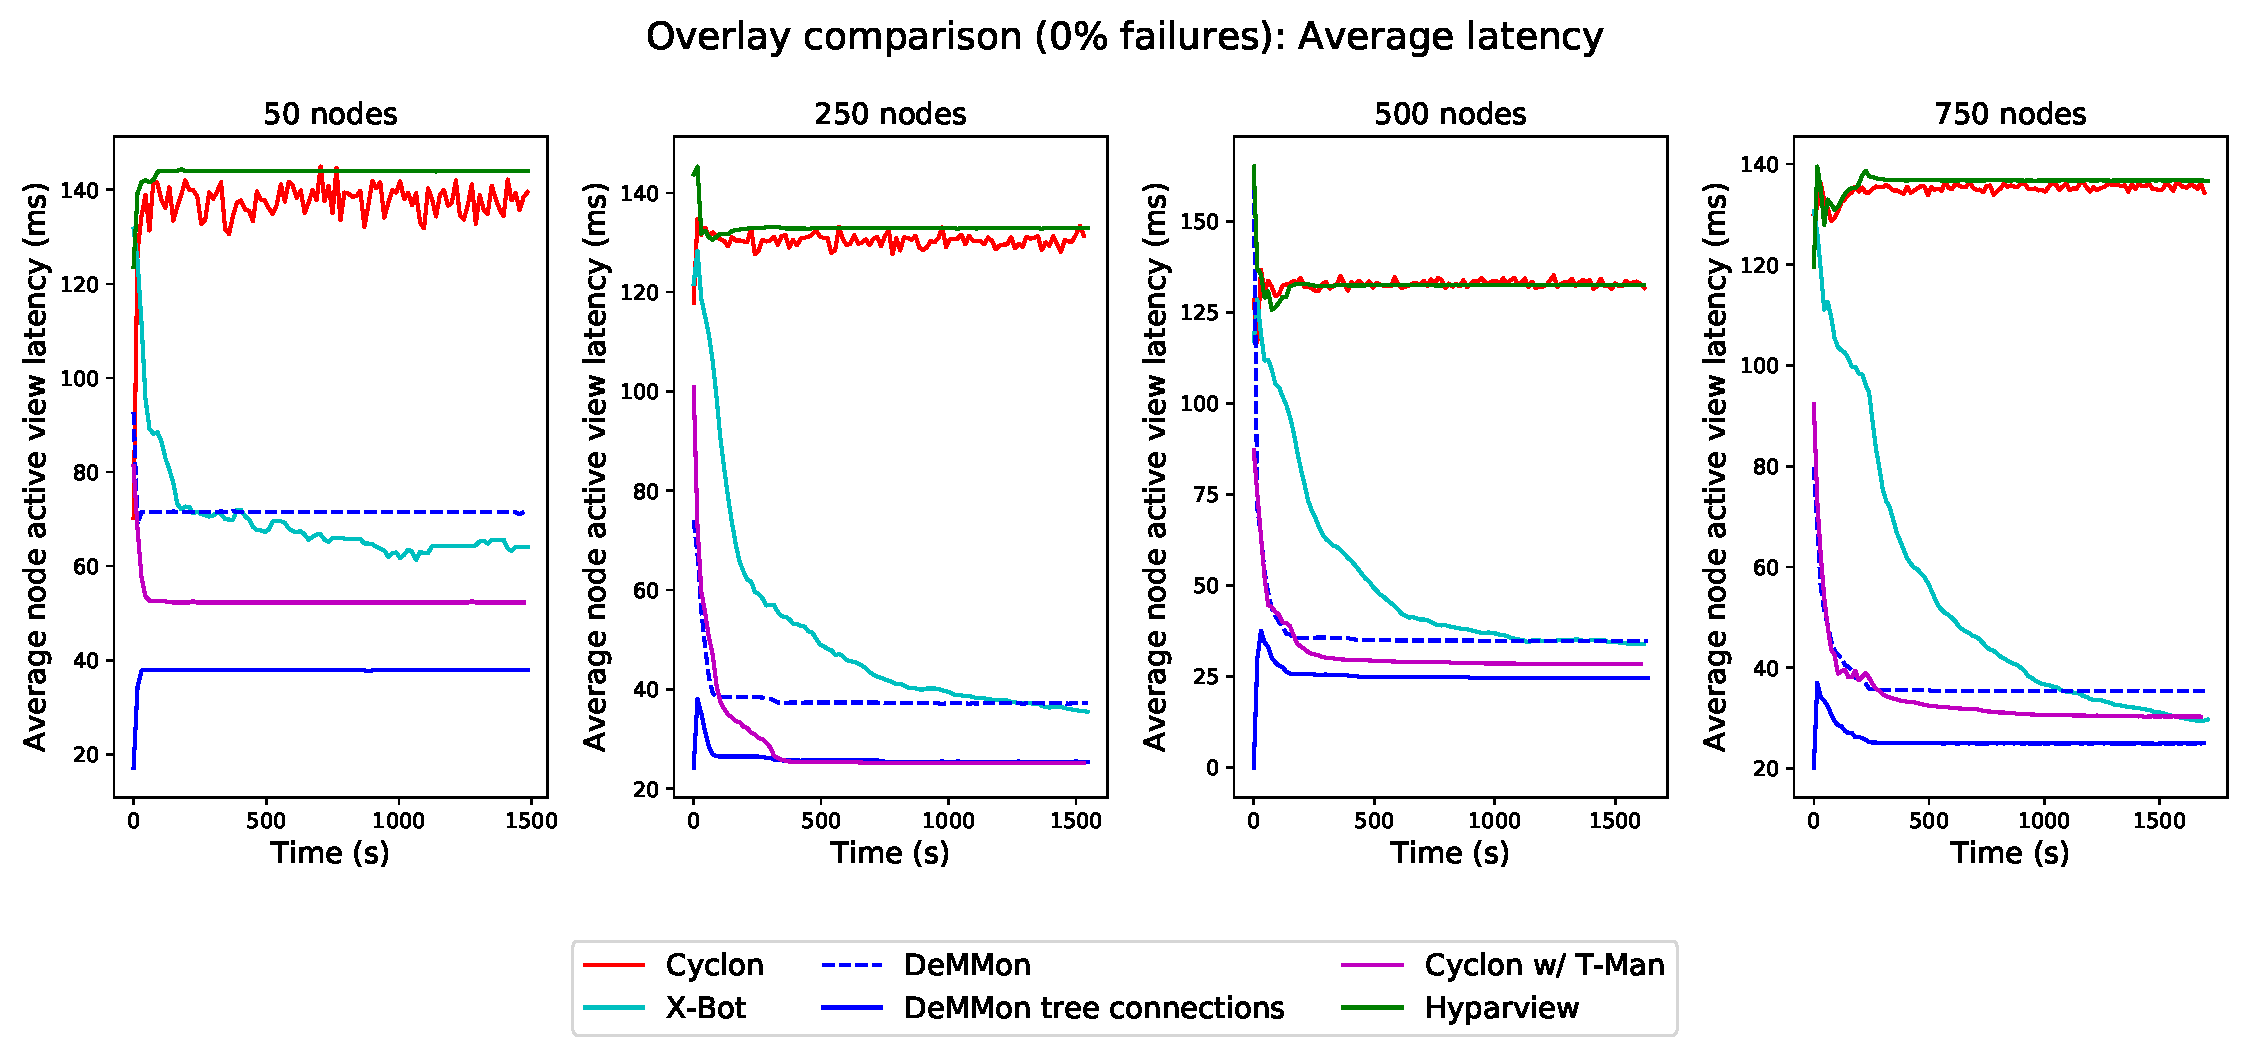
\includegraphics[width=\linewidth]{Chapters/evaluation/figures/membership/membership_lat_over_time_0_failures.pdf}
    \caption{Average latency per node in established networks}
    \label{fig:overlay_proto_res_net_building:0_failures_lat}
\end{figure}


\begin{figure}
    \centering
    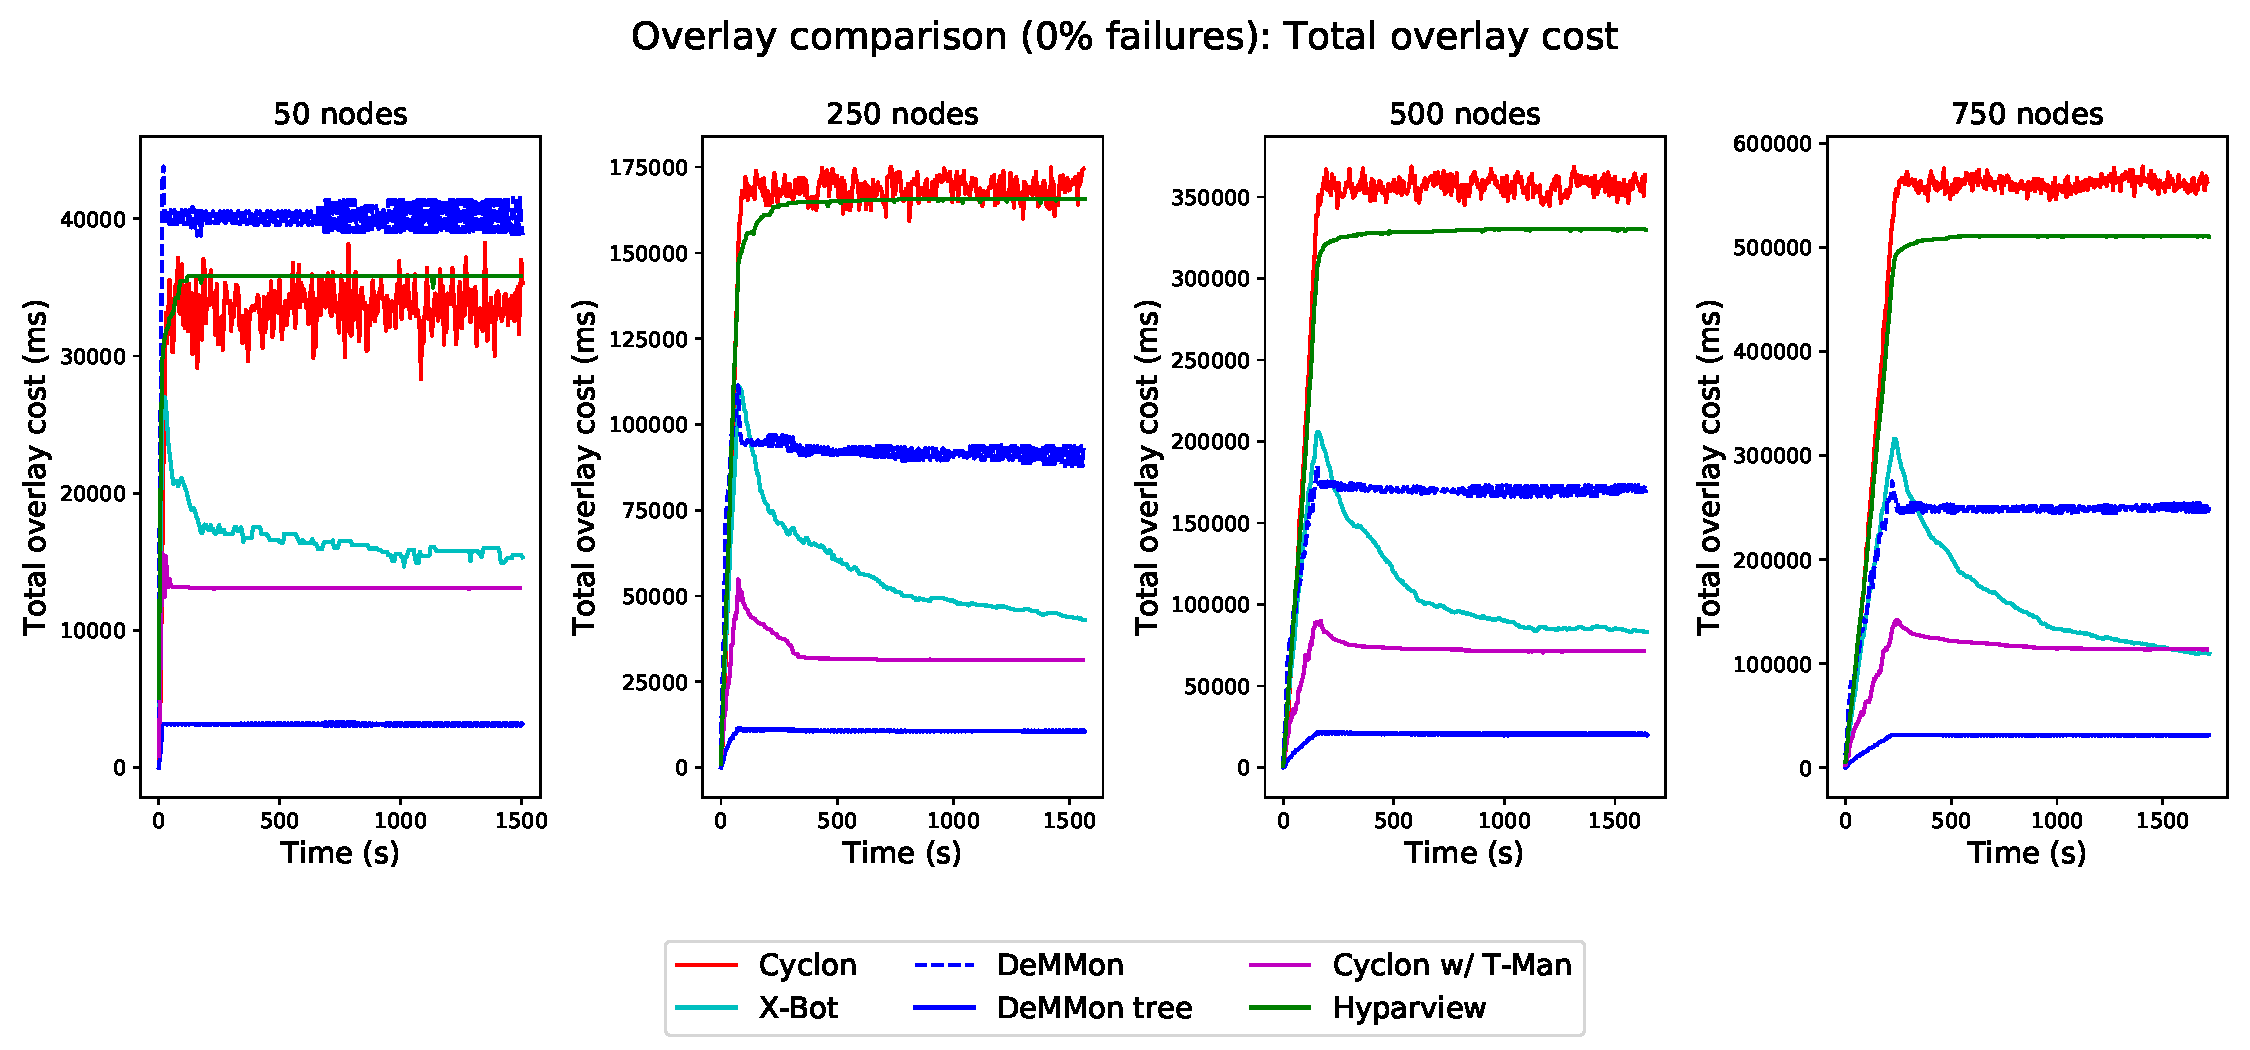
\includegraphics[width=\linewidth]{Chapters/evaluation/figures/membership/membership_total_lat_over_time_0_failures.pdf}
    \caption{Total network cost (in latency)}
    \label{fig:overlay_proto_res_net_building:0_failures_lat_total}
\end{figure}

In the graphs displayed in figures \ref{fig:overlay_proto_res_net_building:0_failures_lat} and \ref{fig:overlay_proto_res_net_building:0_failures_lat_total}, we may observe the results pertaining to the average latency of a connection in the overlay and the total cost of the established overlay networks for the experiment with no failures, respectively. For both of these graphs, we show the results obtained from both the baseline protocols and the DeMMon protocol. In the case of DeMMon, we make a distinction between two latency values, the first (represented by a blue, continuous, line) represents the results relative to all connections of all nodes, the second value (represented by a blue dashed line) represents the cost of the ``vertical'' connections of the DeMMon tree (the parent and children of each node), essentially excluding the siblings of each node from the results. We made this distinction for two reasons: first, as the DeMMon protocol only performs optimizations to improve the parent connection, we believe it is important to see the correlation between improving the parent connections to the sibling latencies. The second reason to make this distinction, is due to the fact that these connections are significantly more used when compared with the sibling connections, namely for for network maintenance, information dissemination and in-transit aggregation. The results displayed in these graphs (\ref{fig:overlay_proto_res_net_building:0_failures_lat} and \ref{fig:overlay_proto_res_net_building:0_failures_lat_total}) show that both Hyparview and Cyclon converge to a similar average latency value, which corresponds to the average of all connections of the latency matrix. This is expected, as these protocols do not attempt to perform optimizations in regard to the network latency. The results also show that the devised protocol is the fastest to converge to its lowest latency value, and that X-Bot is the slowest, not converging to a final value in a test of 25 minutes. We believe this occurs because X-Bots' overlay improvements are performed using 7 messages, contrasting heavily with DeMMons' 2 required messages, and T-Mans' 0 required messages. While the total and average latency of the DeMMon overlay is not the lowest in any of the displayed results, when comparing only the parent and children connections, DeMMon reaches a total latency cost lower than any other tested protocol. This is important given that, as previously mentioned, these connections are the ones most used when performing overlay improvements and maintenance, information dissemination and in-transit aggregation. 

\begin{figure}
    \centering
    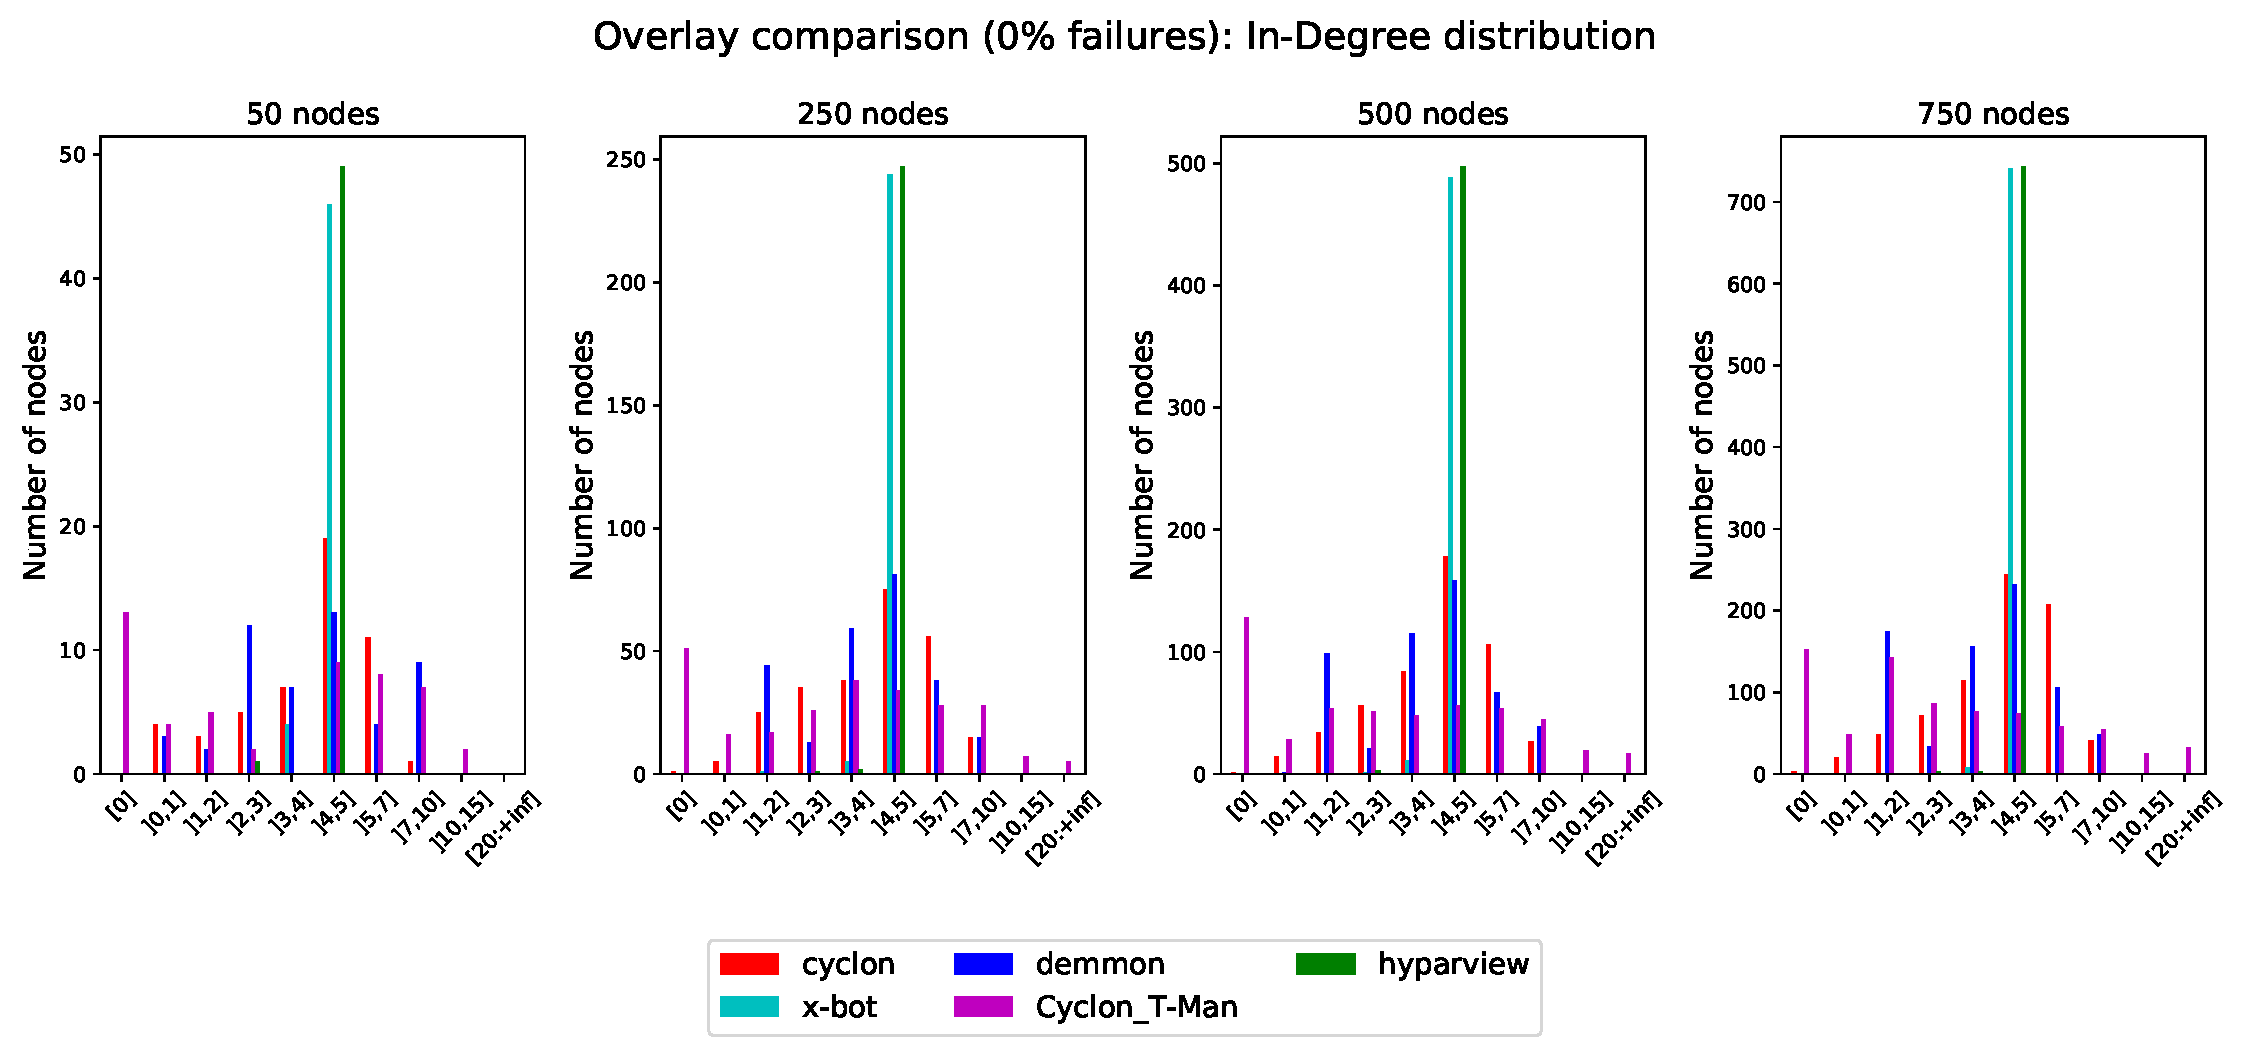
\includegraphics[width=\linewidth]{Chapters/evaluation/figures/membership/membership_inDegree_0_failures.pdf}
    \caption{Node in-degree}
    \label{fig:overlay_proto_res_net_building:0_failures_inDegree}
\end{figure}

It is important to mention that, while T-Man is the protocol that reaches the lowest overall and average latency in the conducted tests, it does so disregarding the fact that nodes may become disconnected from overlay, which as we will observe further, prevents this protocol from being suitable for reliable message dissemination. This may be observed in fig. \ref{fig:overlay_proto_res_net_building:0_failures_inDegree}, which shows the in-degree (the number of incoming connections for each node) for all nodes participating in the network, these results pertain to the last observed configuration of the network before the experiment finished. They show that T-Man, at multiple node counts, possesses nodes with 0 incoming connections, which are effectively isolated from the network. While still analyzing the in-degree results, we observe that both X-Bot and Hyparview have a fixed number of incoming connections, which stems from the use of bidirectional connections, while Cyclon has varied numbers of incoming connections ranging from 10 to 1, which occurs due to the shuffle mechanisms of the active connections. In the case of DeMMon, the values range from 2 to 10 incoming connections, which is expected given the configuration parameters of a minimum number of children of 2, and a maximum number of children of 5.


\begin{figure}
    \centering
    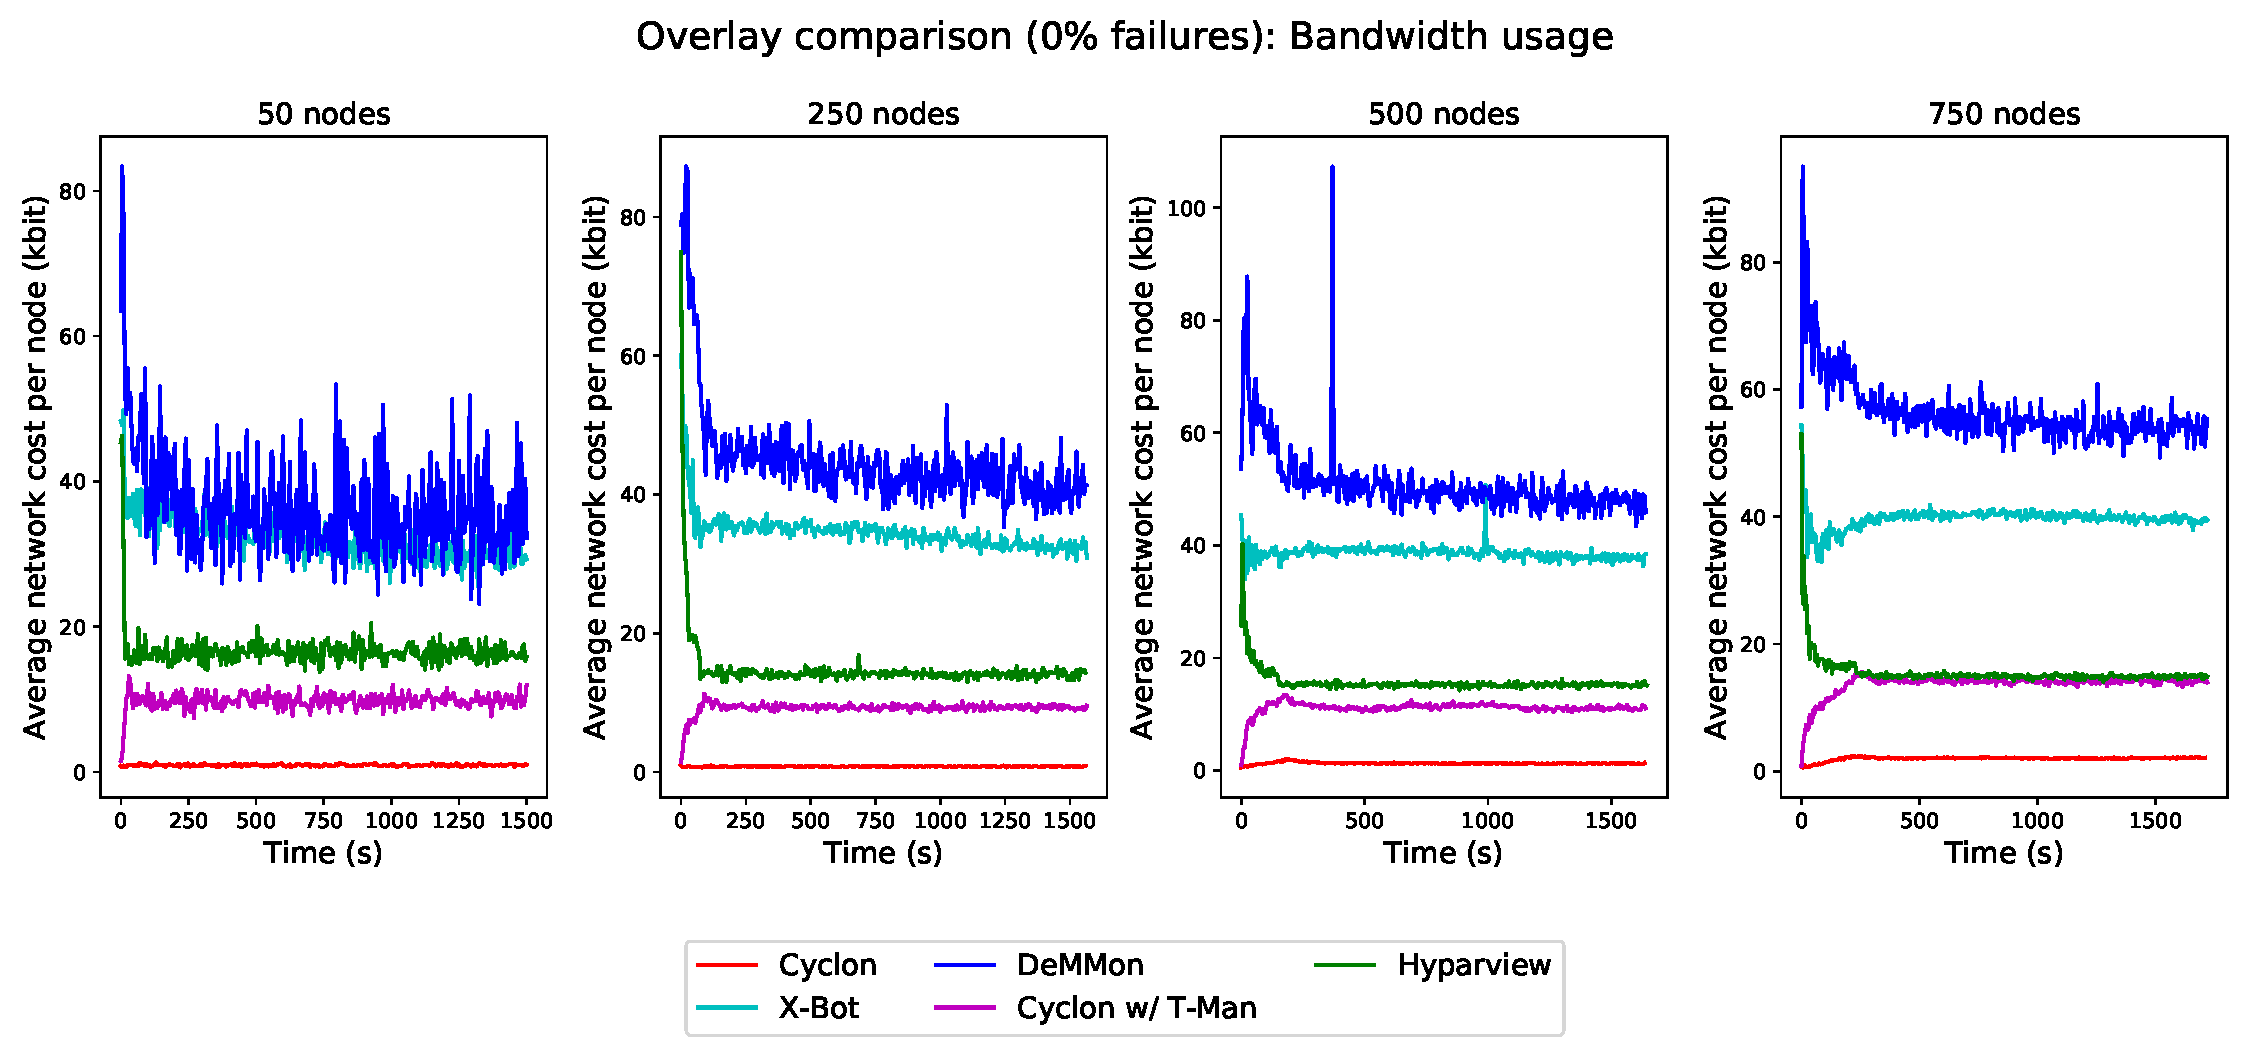
\includegraphics[width=\linewidth]{Chapters/evaluation/figures/membership/membership_bw_over_time_0_failures.pdf}
    \caption{Protocol bandwidth cost}
    \label{fig:overlay_proto_res_net_building:0_failures_BWUsage}
\end{figure}

Finally, still regarding the experiments without node failures, we show, in figure \ref{fig:overlay_proto_res_net_building:0_failures_BWUsage}, the average network cost (in kbit/5s) incurred by each node running the experiments. This graph shows that DeMMons' overlay protocol, on average, spends more bandwidth to build and maintain the network structure, we believe this is because DeMMon exchanges more information periodically with peers in the active view to maintain and improve the network structure when compared to the other protocols. Conversely, the protocol which uses the least amount of bandwidth is Cyclon, as its shuffle mechanism is relatively inexpensive and the protocol possesses no other mechanisms that incur networking costs. Although protocols have varied networking costs, we believe that even DeMMon, that uses the most bandwidth, is relatively inexpensive when compared with the bandwidth standards at the time of writing this work.

\begin{figure}
    \centering
    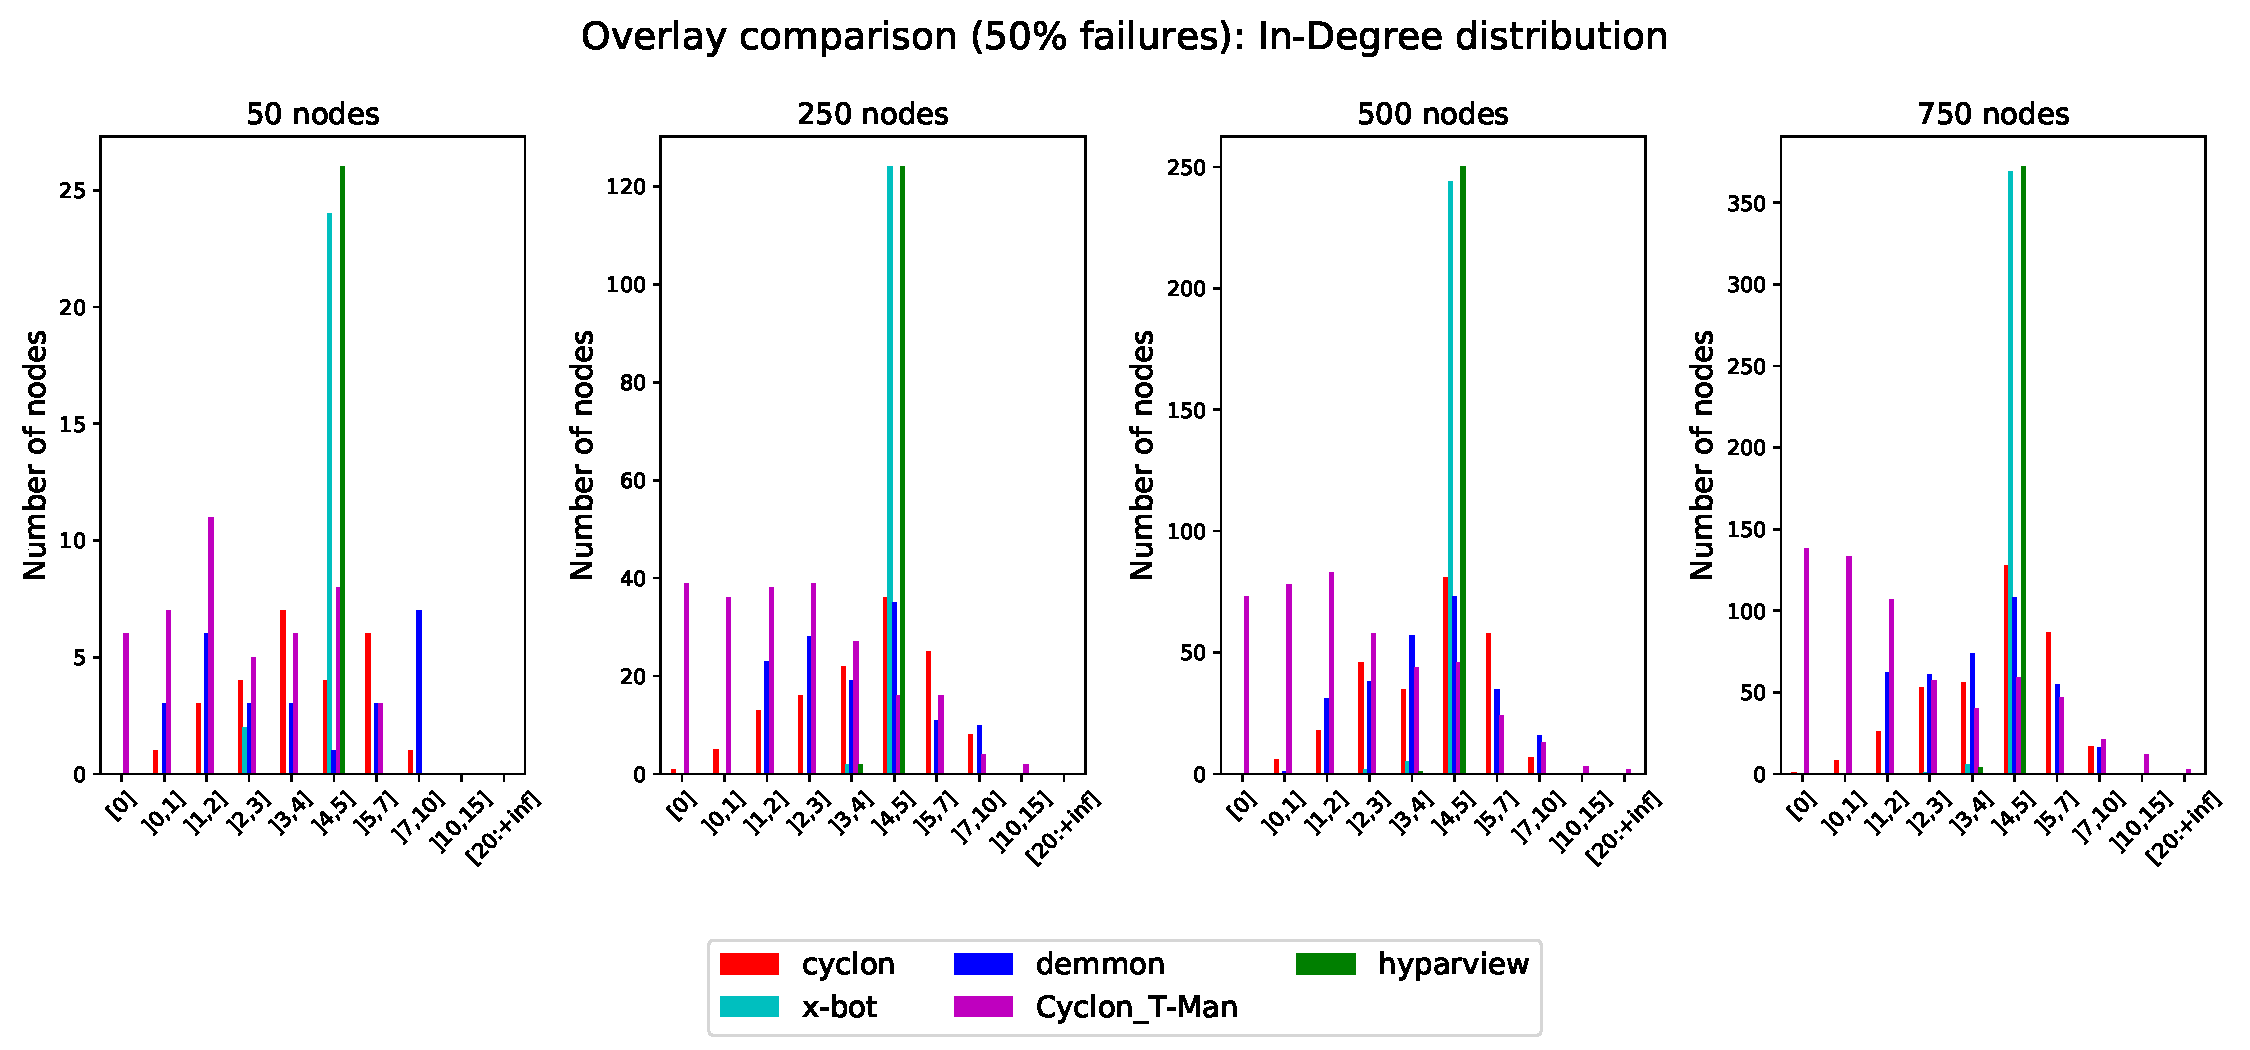
\includegraphics[width=\linewidth]{Chapters/evaluation/figures/membership/membership_inDegree_50_failures.pdf}
    \caption{Node in-degree (50\% failures)}
    \label{fig:overlay_proto_res_net_building:50_failures_inDegree}
\end{figure}

Provided with the result analysis for the experiments with no failures, we now provide the results for the in-degree distribution of the protocol in a scenario with failures. This experiment attempts to test the fault tolerance of the protocols by first establishing the network, and during the middle of the experiment, induce a failure of 50\% of the nodes. The objective of this experiment was to test if any node became isolated from the network after the failures. Results from this experiment may be observed in figure \ref{fig:overlay_proto_res_net_building:50_failures_inDegree}, where it is observable that, for all tested protocols except T-Man, no nodes became isolated, allowing us to conclude that both the devised protocol and the tested baselines can recover from faults effectively.

As previously mentioned, the applicability of our solution was tested in two different aspects: the first was the process of building and maintaining the overlay network, which was covered in the previous paragraphs. The second evaluated aspect is information dissemination (via message broadcasting), which we will now cover in the following subsection.

\subsection{Information dissemination} \label{results:inf_diss}

The second set of conducted experiments, as mentioned previously, intends to test the applicability of the devised membership protocol in an information dissemination scenario. To do so, we tested it against the same set of baseline protocols used in the previous experiments enriched with two message dissemination protocols: the first is a simple flood protocol, where if a node wishes to broadcast a message, it sends that message to every peer in its active view, then, nodes that receive this message, propagate it to every neighbour if they have not done so previously (excluding the sender). The second used dissemination protocol was PlumTree \cite{plumTree}, which is a dissemination protocol that builds a dissemination tree based on the paths taken by the broadcast messages.

The reasoning behind this choice of dissemination protocols was to provide a more comprehensive comparison of DeMMon with the remaining protocols. As the simple flood generates redundant messages when compared to dissemination primitives tree structures, we included an implementation of a dissemination protocol that also employs a tree for dissemination of messages. It is important to mention that, when testing the PlumTree protocol, in order to establish the initial tree structure, a single node first starts the dissemination of its messages a minute earlier than other nodes. For both of these comparisons, DeMMon is set up with a dissemination protocol similar to the simple flood protocol, however only using its vertical connections (parent and children).

Similarly to the first set of experiments, we conducted multiple tests with 50, 250, 500 and 750 nodes during 15 minute periods, for all these node numbers, we also tested failure rates of 0 and 50\%. For each of these combinations, we varied the number of messages each node emitted until all protocols reach their saturation point. While doing the tests, we extracted the following metrics: (1) the reliability of the messages, i.e. what is the average percentage of nodes that receive the emitted broadcast messages ; (2) the maximum message throughput reached by every protocol in a 30-second window, (3) the average latency taken by messages until they reach other nodes, and (4) the bandwidth usage of each of the protocols. 

\begin{figure}[htbp]
    \centering
    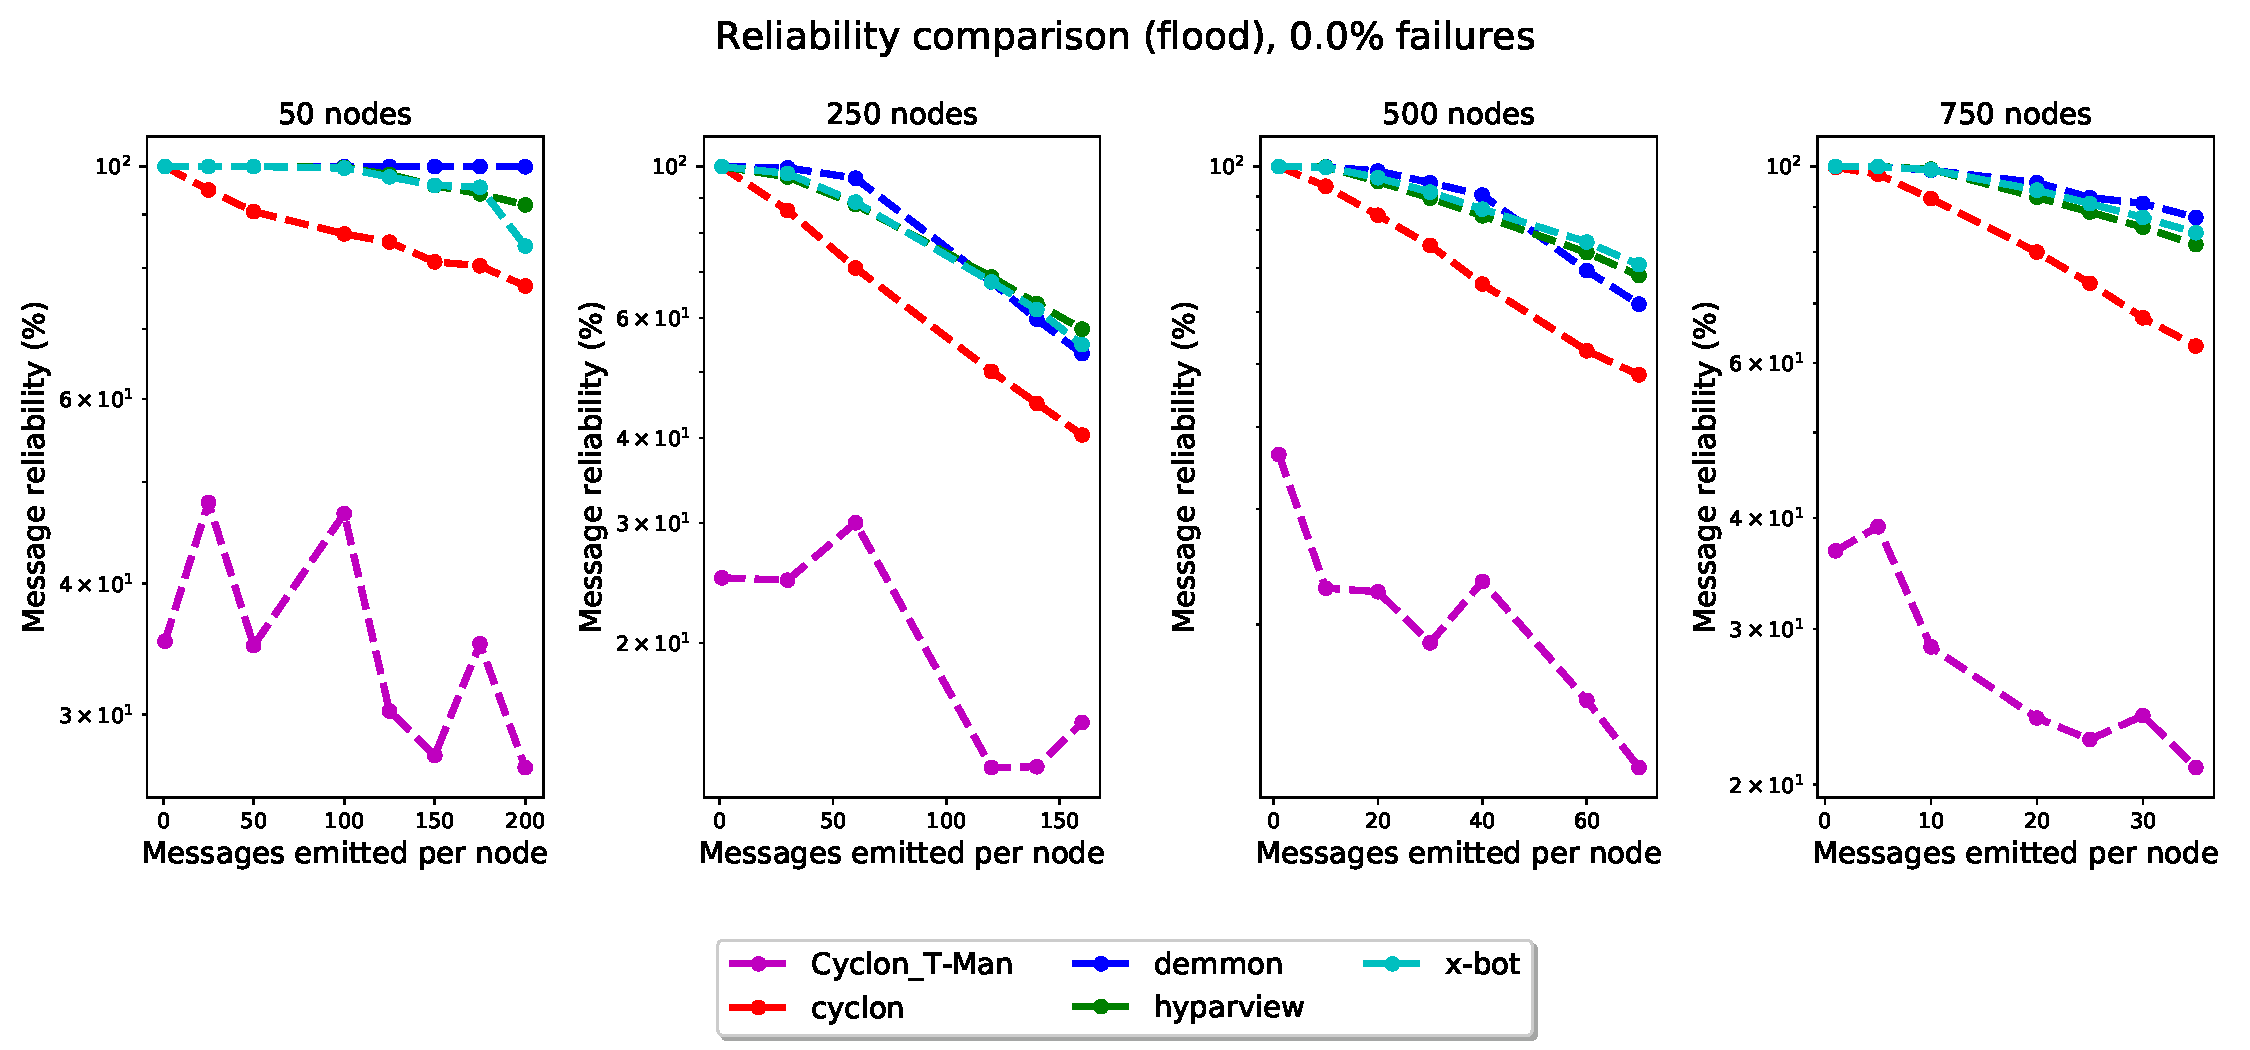
\includegraphics[width=\linewidth]{Chapters/evaluation/figures/flood/flood_0.0_failures_reliability.pdf}
    \caption{Average message reliability in simple flood scenario (0\% failures)}
    \label{fig:overlay_proto_res_msg_diss:0_failures_reliability_flood}
\end{figure}

\begin{figure}[htbp]
    \centering
    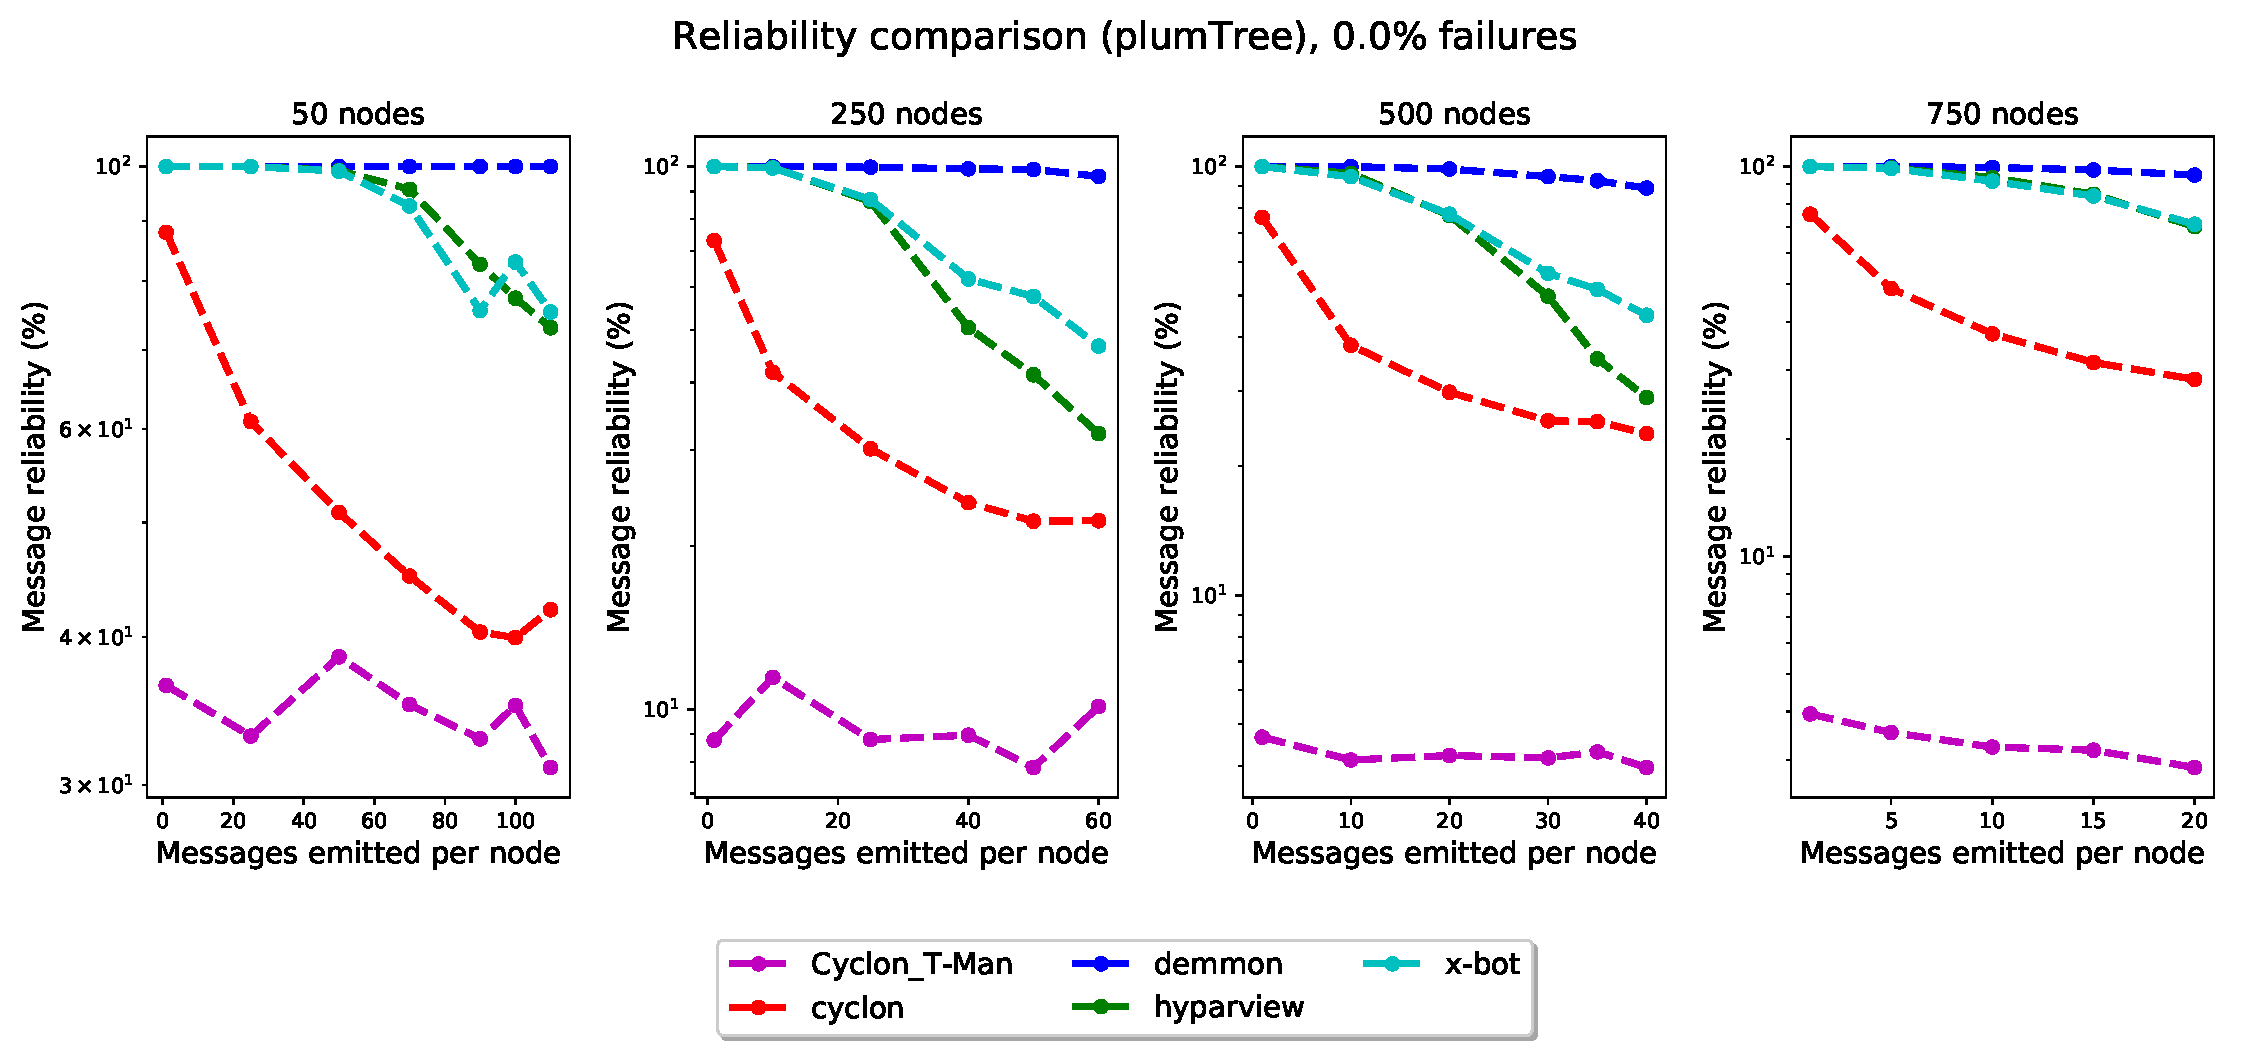
\includegraphics[width=\linewidth]{Chapters/evaluation/figures/flood/plumTree_0.0_failures_reliability.pdf}
    \caption{Average message reliability in PlumTree scenario (0\% failures)}
    \label{fig:overlay_proto_res_msg_diss:0_failures_reliability_plumTree}
\end{figure}

Figures \ref{fig:overlay_proto_res_msg_diss:0_failures_reliability_flood} and \ref{fig:overlay_proto_res_msg_diss:0_failures_reliability_plumTree} show the obtained results regarding the message reliability during the experiments for both the simple flood and PlumTree experiments with 0 failures. As we may observe, in general, the saturation point for all protocols using PlumTree tends to be earlier (in terms of emitted messages per node) than the simple flood protocol. We believe this occurs because the PlumTree protocols' tree becomes unstable whenever certain nodes become a bottleneck to the messages being propagated using the tree (because their bandwidth capacity is exceeded). Whenever this occurs, as certain messages get delayed, the tree structure becomes unstable (as the order of delivery of messages is what defines the dissemination tree structure). Whenever this occurs, the tree repair procedure is triggered, however as multiple nodes emit new messages and other nodes can become saturated while performing this mechanism, the tree structure may never reconverge until all messages are delivered (and nodes stop being saturated). Until this occurs, the protocol essentially becomes a push-pull gossip protocol, which has lower performance in our experiments in terms of reliability because message delivery requires 2 messages, incurring additional networking costs (and the tests end before the protocol has delivered all emitted messages).

In addition to the previously mentioned reasons, in an occasion where a node has received an IHAVE message for a certain message and at that moment happens to have available upload bandwidth, but its download capacity is all taken up by incoming traffic, this node will periodically emit GRAFT messages to the sender of the IHAVE message, which, in turn, will reply with the broadcast messages that will only be received after a large time frame. During this time frame, there may be multiple redundant GRAFT and IHAVE messages being emitted, which results in the system possibly becoming even more saturated, which causes the tree to become even more unstable. The devised overlay protocol, although it also uses a tree structure, its tree is not defined by the propagations of broadcast messages and consequently is not as susceptible to instability in conditions where the network is saturated, consequently achieving higher reliability in higher message counts. 

We may observe that both the Cyclon and T-Man tend to perform worse in general regard to reliability when compared to DeMMon, Hyparview and DeMMon, which we believe, in the case of T-Man, to occur because there are nodes with 0 incoming connections and consequently do not receive any broadcast messages from other nodes. In the case of Cyclon, we believe the lower reliability value is attributed to the use of UDP as its communication medium, which means that whenever the data channels become saturated, many of the broadcast messages are lost, contrary to DeMMon, Hyparview and X-BOT, that use TCP and consequently do not drop messages in congestion periods. Finally, we believe that both Cyclon and T-MAN, when paired with PlumTree, also have lower reliability because this protocol requires bidirectional connections to perform optimally, which are not guaranteed in either of these protocols. 

In regard to the simple flood experiment (fig. \ref{fig:overlay_proto_res_msg_diss:0_failures_reliability_flood}), DeMMon tends to perform exceptionally well with fewer node counts, particularly with 50 nodes. We believe this may be due to the height of the DeMMon tree being lower, as when the tree height is smaller, the number of descendants for each node is fewer, which in turn means that when a certain node becomes saturated, fewer nodes are impacted by it. In higher node counts, DeMMon performs in line with both Hyparview and X-Bot. We believe this happens because the tradeoffs of having a tree (a single node possibly becoming a bottleneck for many other nodes in the system) tend to impact the system the same amount that sending multiple redundant messages does. 

\begin{figure}[htbp]
    \centering
    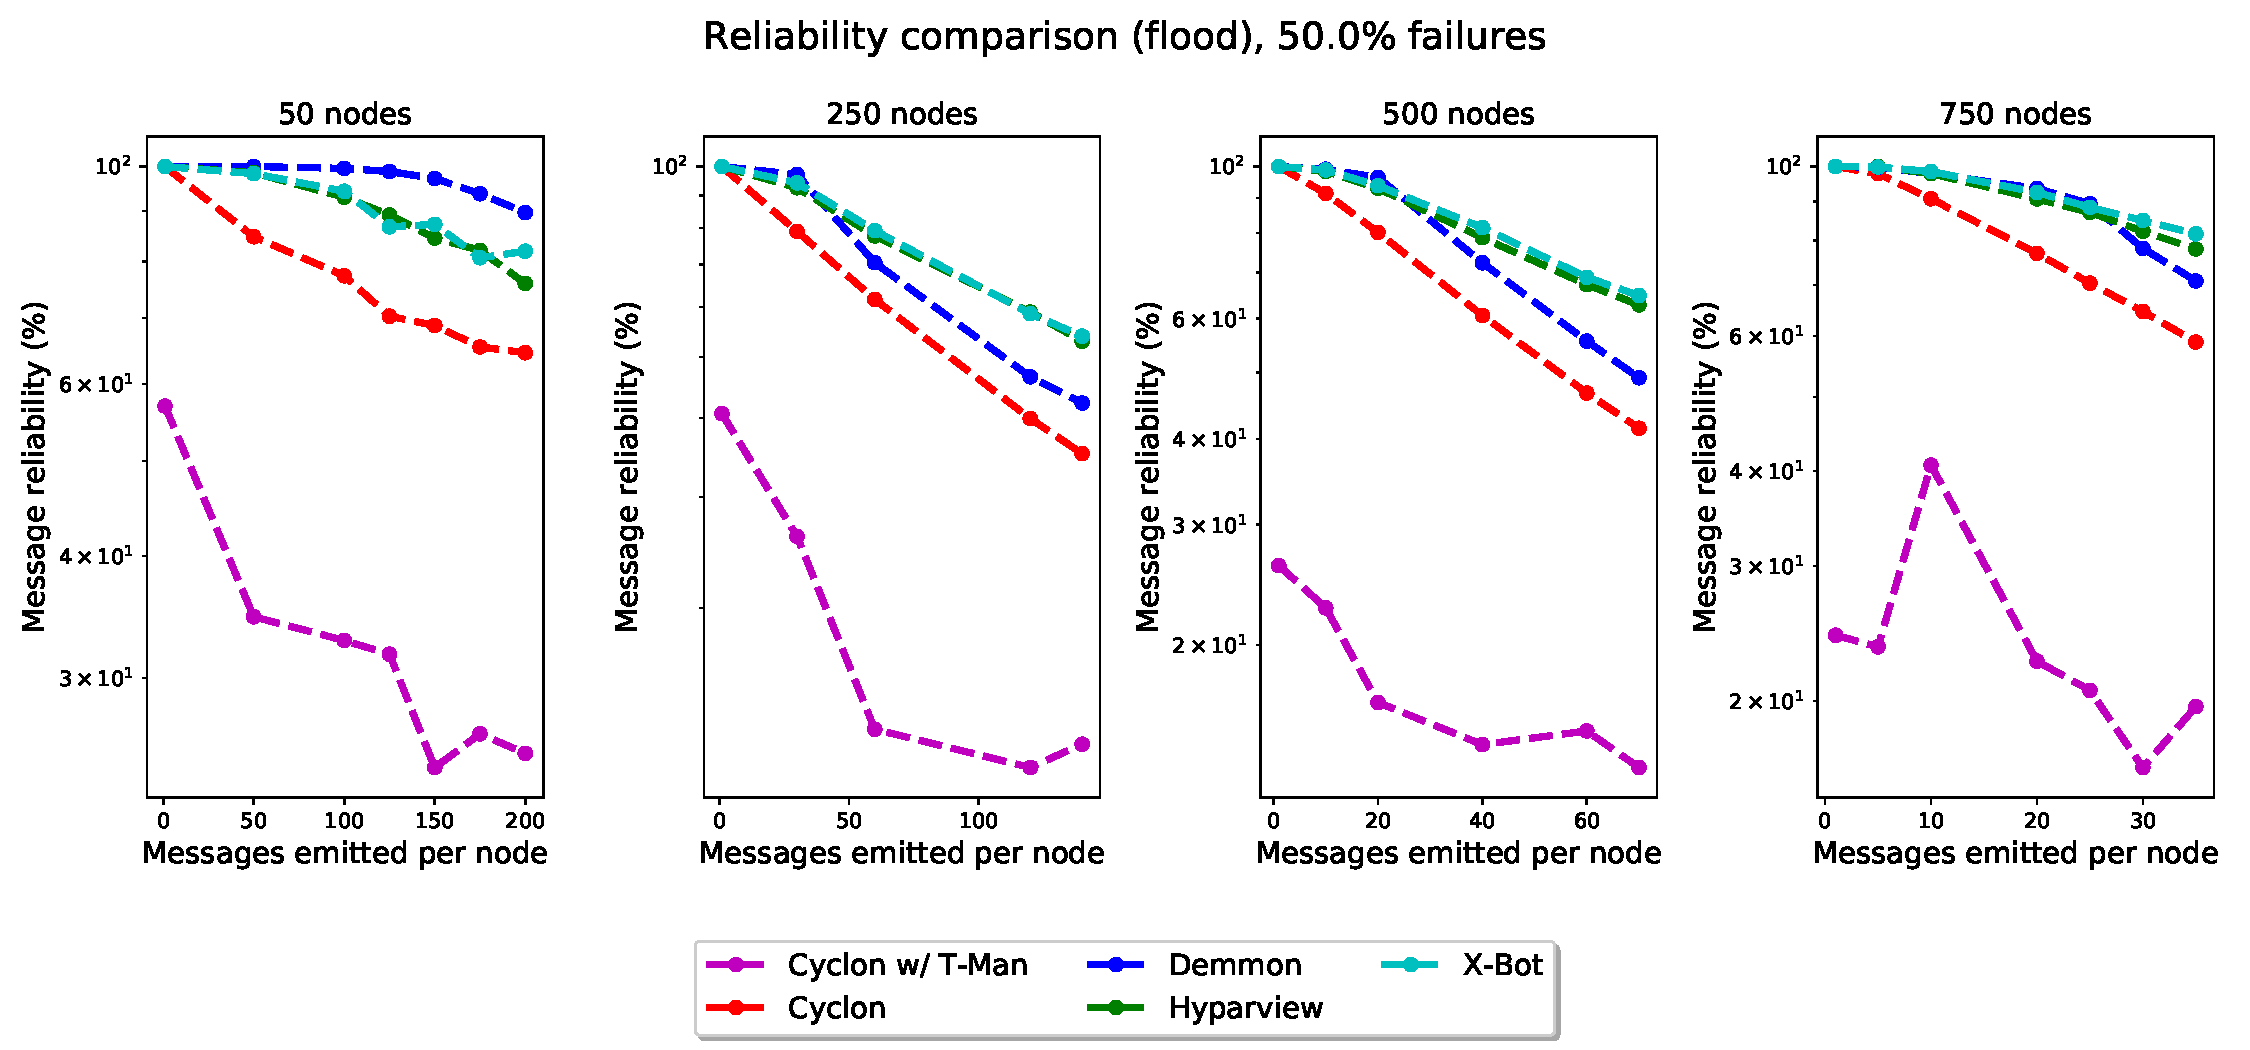
\includegraphics[width=\linewidth]{Chapters/evaluation/figures/flood/flood_50.0_failures_reliability.pdf}
    \caption{Average message reliability in simple flood scenario (50\% failures)}
    \label{fig:overlay_proto_res_msg_diss:50_failures_reliability_flood}
\end{figure}

\begin{figure}[htbp]
    \centering
    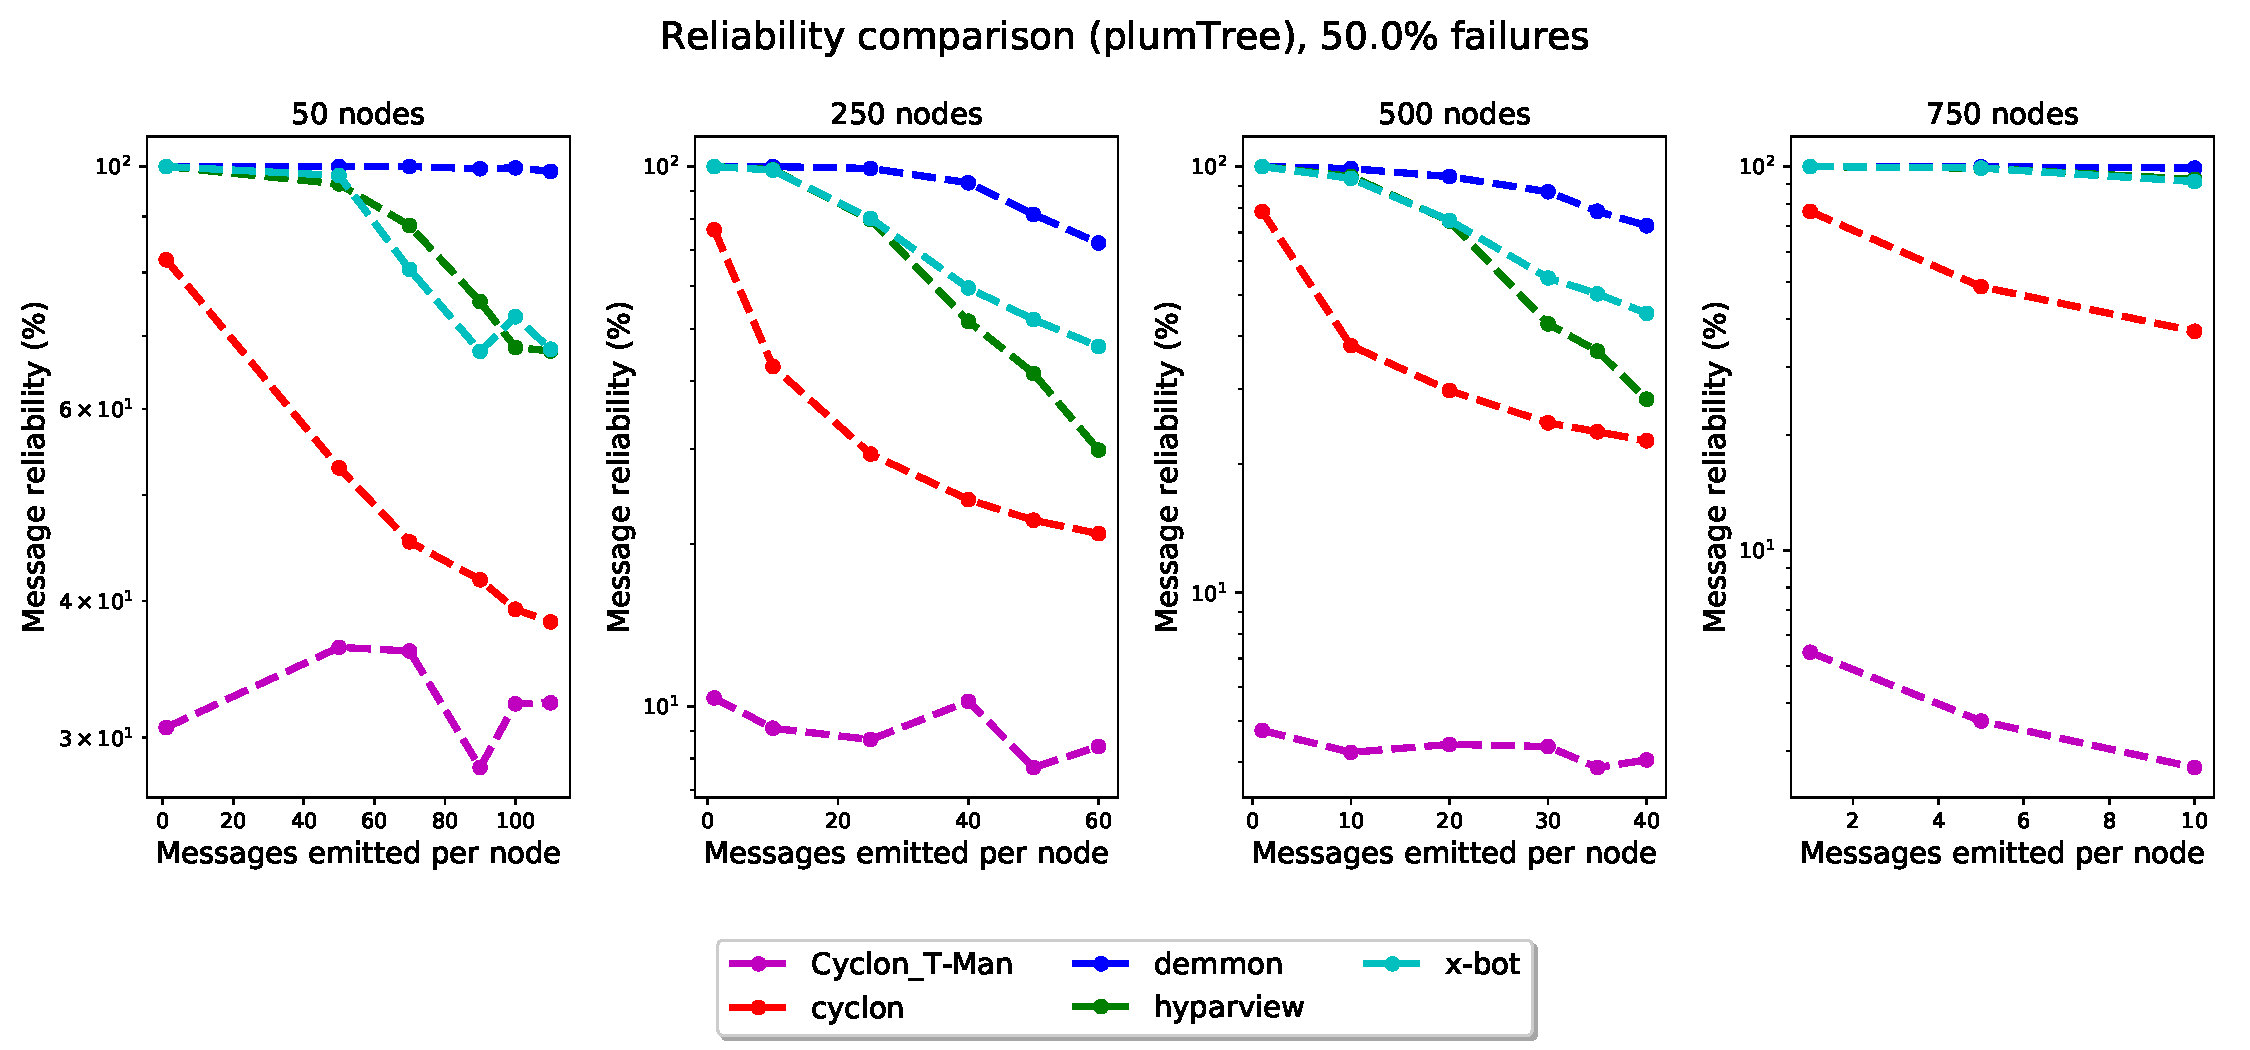
\includegraphics[width=\linewidth]{Chapters/evaluation/figures/flood/plumTree_50.0_failures_reliability.pdf}
    \caption{Average message reliability in PlumTree scenario (50\% failures)}
    \label{fig:overlay_proto_res_msg_diss:50_failures_reliability_plumTree}
\end{figure}

In the case of scenarios with induced failures (figures \ref{fig:overlay_proto_res_msg_diss:50_failures_reliability_flood} and \ref{fig:overlay_proto_res_msg_diss:50_failures_reliability_plumTree}), we observe a similar trend in regard to the PlumTree experiments, with DeMMon achieving higher reliability values. However, in the simple flood experiments, we observe that DeMMon achieves a lower reliability value when under congestion, we believe this occurs because as the failures are occurring, if the nodes are saturated, the failure recovery mechanisms may take a long time frame to execute, and during this period nodes are disconnected from the remaining overlay and consequently do not receive or send message to or from any node which is not their descendant, leading to a lower reliability value.

Provided the results from the combination of the baseline protocols with PlumTree consistently performs worse in terms of reliability (when the network is saturated) when compared to employing only a simple flood protocol, we now focus on the comparison between DeMMon and the baseline protocols executing the simple flood protocol, however all obtained results are available in annex \ref{annex_1}.

\begin{figure}[htbp]
    \centering
    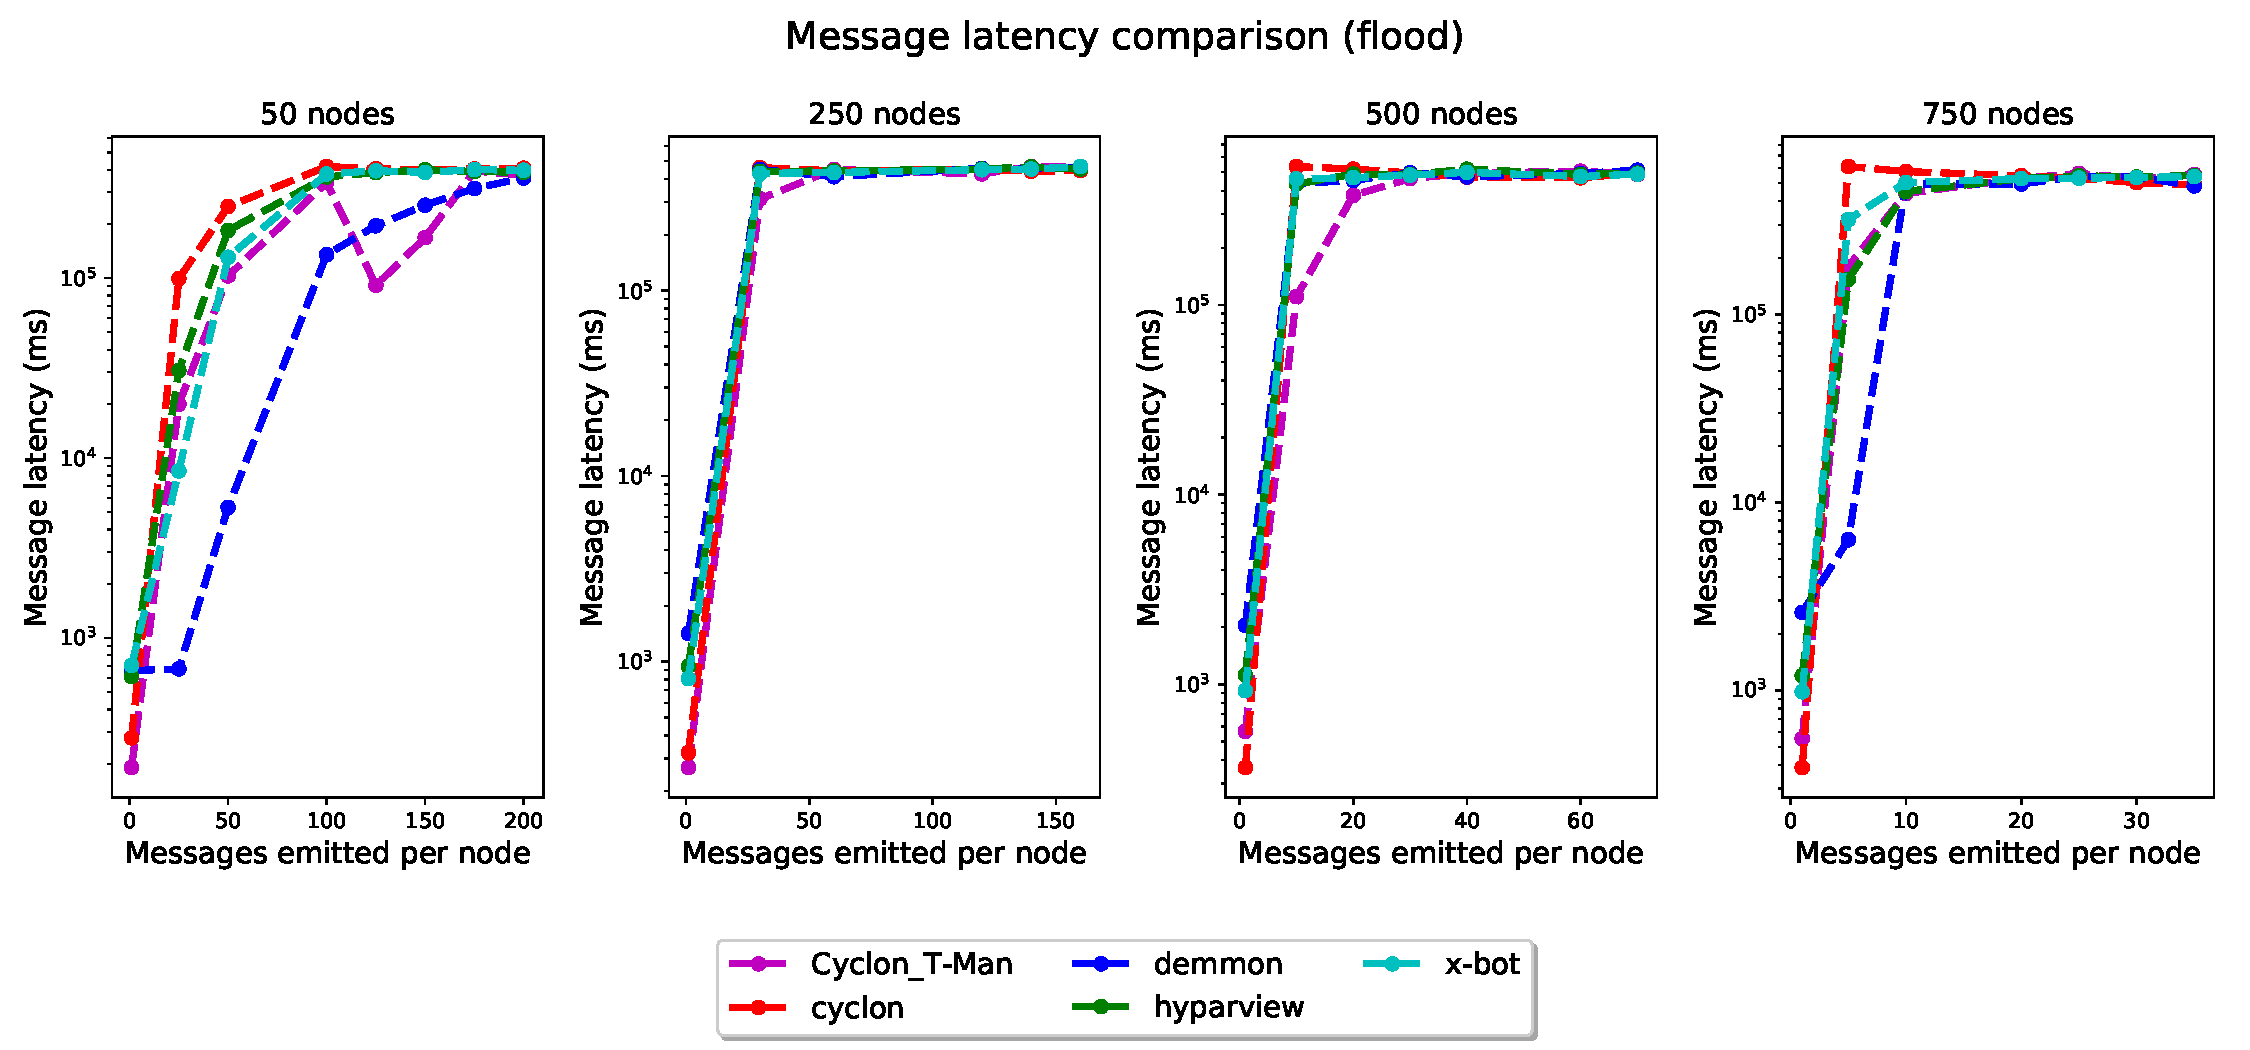
\includegraphics[width=\linewidth]{Chapters/evaluation/figures/flood/flood_0.0_failures_msg_lat.pdf}
    \caption{Average message latency (in ms) in simple flood scenario (0\% failures)}
    \label{fig:overlay_proto_res_msg_diss:0_failures_latency_flood}
\end{figure}

In figure \ref{fig:overlay_proto_res_msg_diss:0_failures_latency_flood}, we may observe the obtained results from collecting the latency between the emission and reception of broadcast messages for each node. The first takeaway from these results is that all protocols plateau at the same latency value, we believe this is due to the fact the the test times are limited to 15 minutes, and whenever the system is saturated, all messages tend to take a similarly long time to be delivered, those which are not delivered are only reflected in the previously discussed reliability graphs (figures \ref{fig:overlay_proto_res_msg_diss:0_failures_reliability_flood}, \ref{fig:overlay_proto_res_msg_diss:0_failures_reliability_plumTree}, \ref{fig:overlay_proto_res_msg_diss:50_failures_reliability_flood}, and \ref{fig:overlay_proto_res_msg_diss:50_failures_reliability_plumTree}). However, for lower message counts, the latency results show that DeMMon tends to achieve lower latency values when compared with the baseline protocols on certain workloads (e.g. low numbers of messages emitted on both the 50 and 750 node graphs) where we believe the simple flood protocol becomes saturated due to the number of redundant messages sent.

\begin{figure}[htbp]
    \centering
    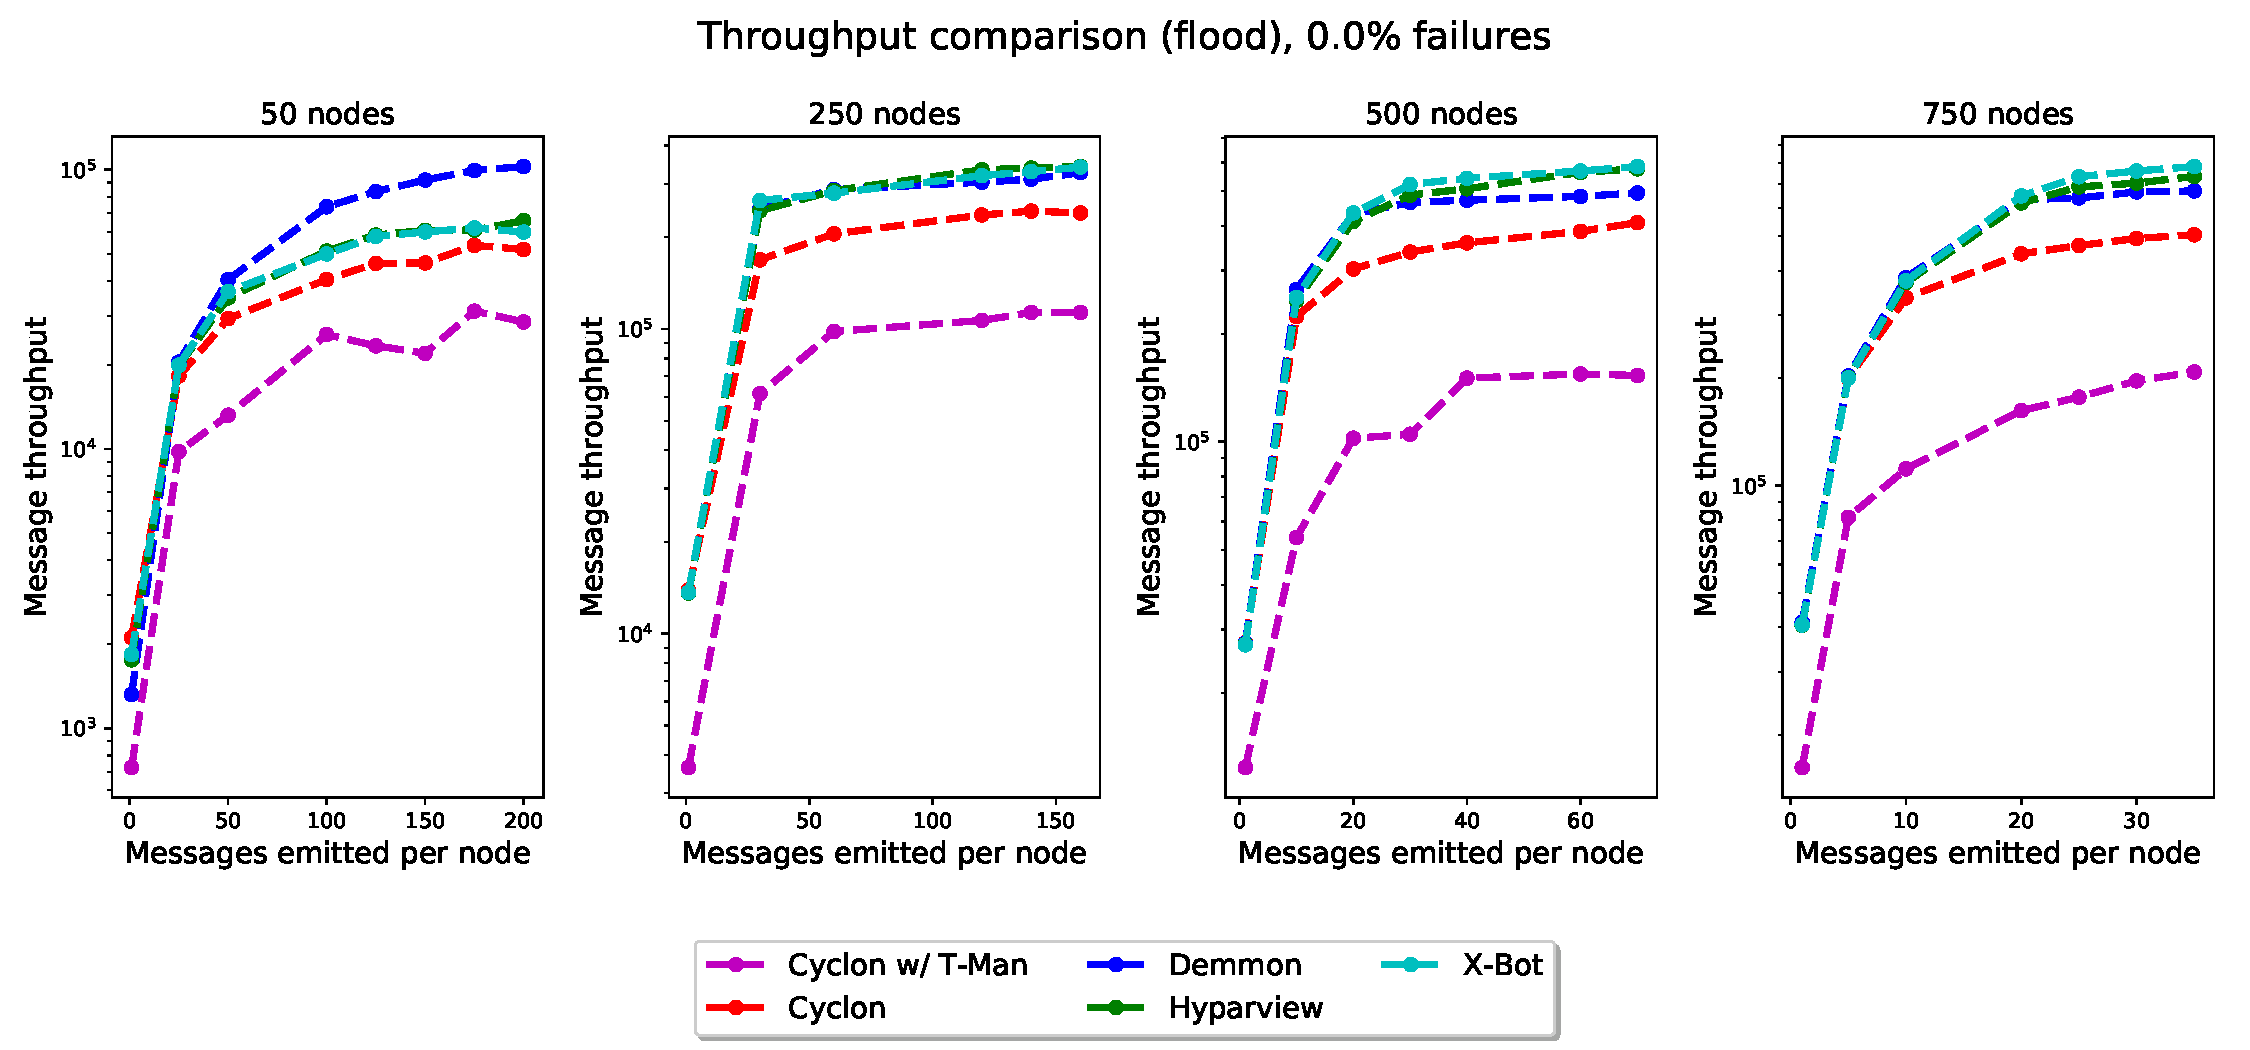
\includegraphics[width=\linewidth]{Chapters/evaluation/figures/flood/flood_0.0_failures_throughput.pdf}
    \caption{Maximum message throughput during experiment (30 second window) in simple flood scenario (0\% failures)}
    \label{fig:overlay_proto_res_msg_diss:0_failures_throughput_flood}
\end{figure}

In figure \ref{fig:overlay_proto_res_msg_diss:0_failures_throughput_flood}, we may observe the obtained throughput across the message dissemination experiments for the simple flood protocol with 0 failures. As we can observe, in lower node counts (i.e. 50 nodes), the throughput achieved by DeMMon surpasses the throughput achieved by the remaining protocols, which also explains the higher values of reliability achieved by DeMMon in these node counts (see fig. \ref{fig:overlay_proto_res_msg_diss:50_failures_reliability_flood}). However, at higher node counts, all protocols tend to plateau at the same throughput, which we believe to be attributed to the fact that, as previously mentioned, the tradeoffs of using a tree (a single node possibly becoming a bottleneck for many other nodes in the system) tends to impact the system the same amount that sending multiple redundant messages does.

\begin{figure}[htbp]
    \centering
    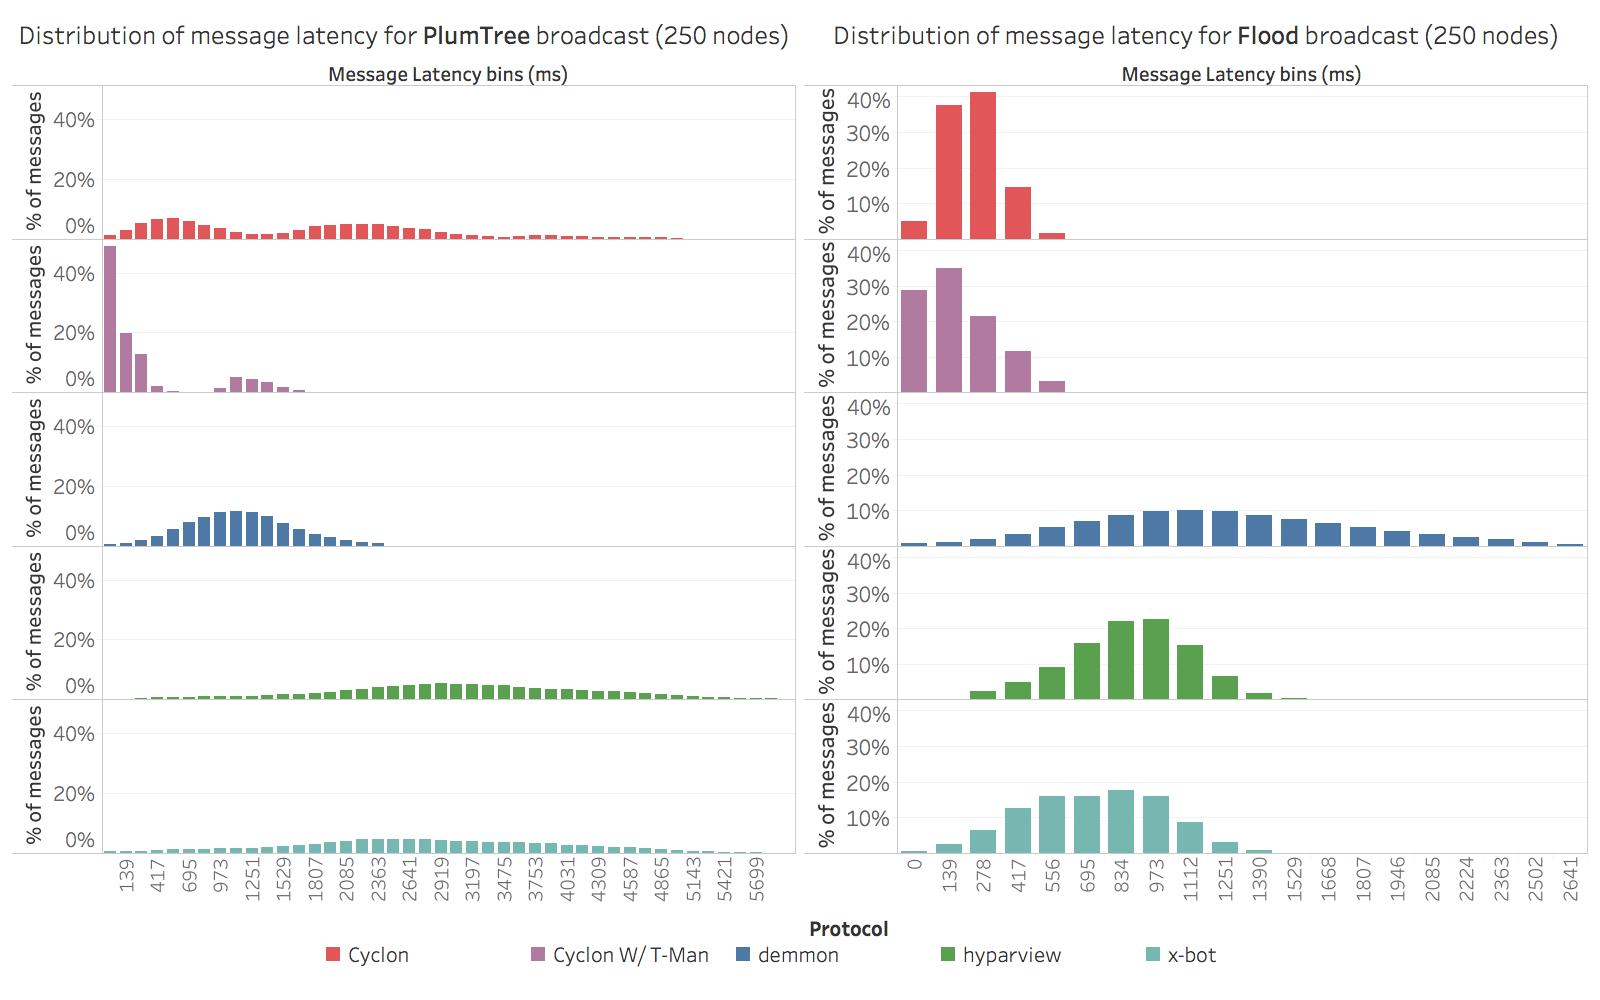
\includegraphics[width=\linewidth]{Chapters/evaluation/figures/flood/Message latency comparison.jpg}
    \caption{Message latency distribution in scenario with low network saturation}
    \label{fig:overlay_proto_res_msg_diss:0_failures_msg_lat_histogram}
\end{figure}


\begin{figure}[htbp]
    \centering
    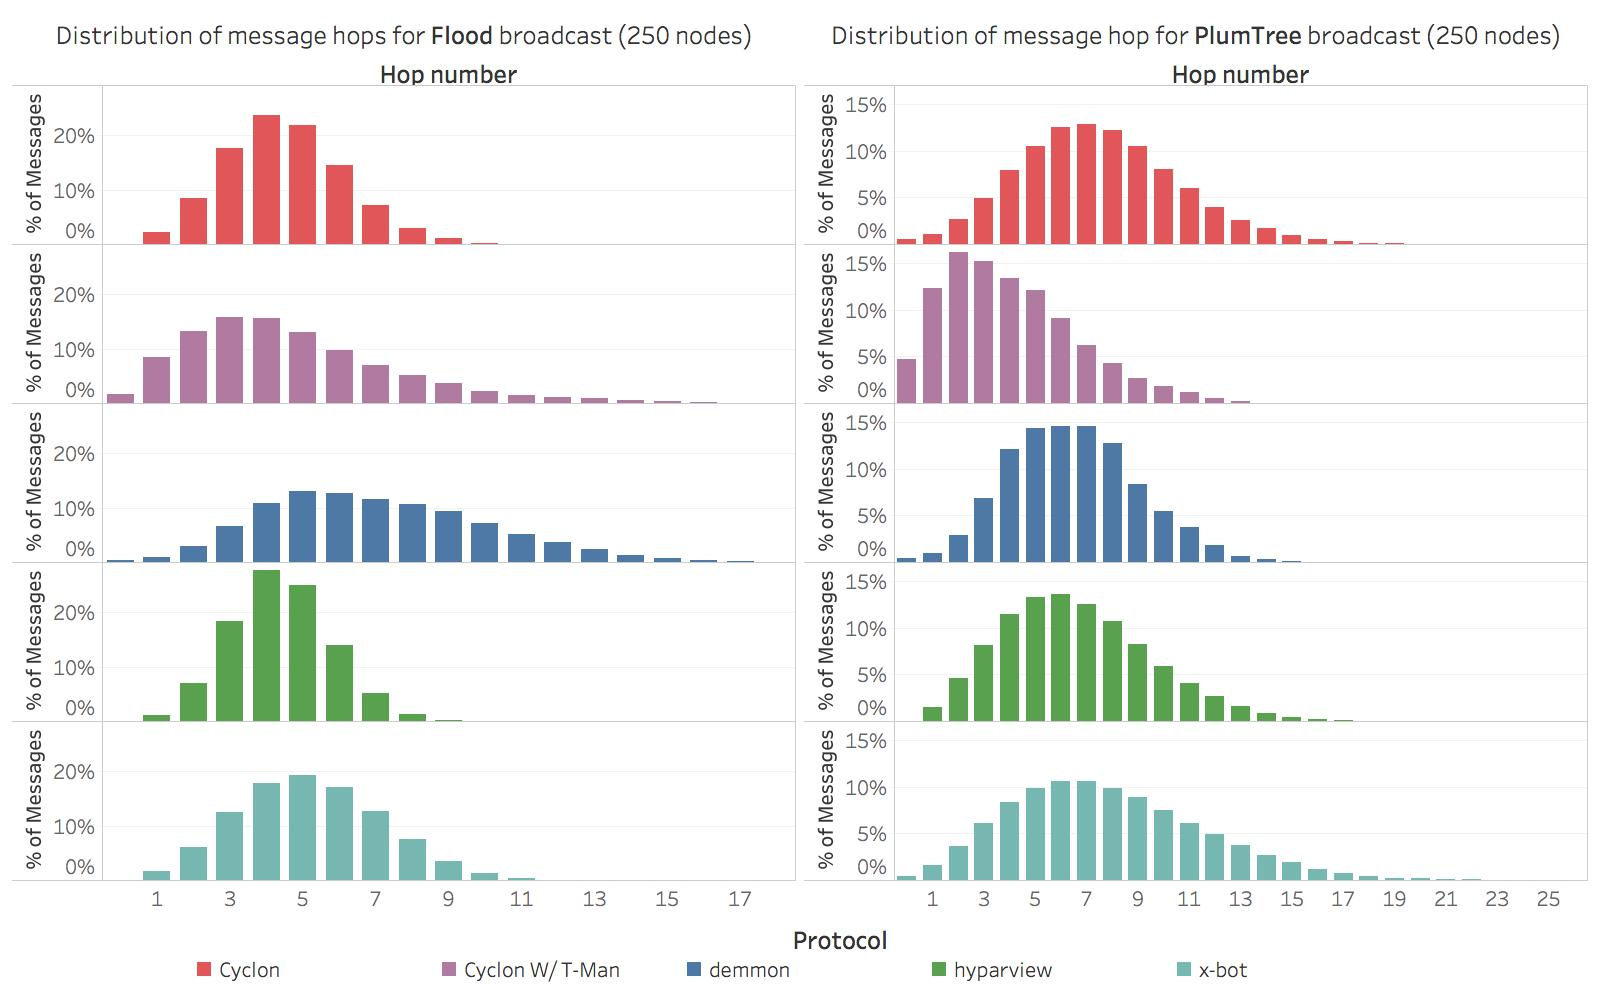
\includegraphics[width=\linewidth]{Chapters/evaluation/figures/flood/Message hop distribution.jpg}
    \caption{Message hop distribution in scenario with low network saturation}
    \label{fig:overlay_proto_res_msg_diss:0_failures_msg_hop_histogram}
\end{figure}

In figure \ref{fig:overlay_proto_res_msg_diss:0_failures_msg_lat_histogram} we compare the baseline protocols with DeMMon in regard to the message latency. These results show the averaged latency distribution for the tests conducted with 250 nodes and one message emitted per node. On the left graph, we may observe the results obtained by the execution of PlumTree with the baseline protocols, while on the right graph, we have the results for the simple flood tests. As we can observe, in general, the message latency obtained by combining simple flood with the baseline protocols tends to be lower in latency when compared with protocols that employ shared trees to disseminate the messages, such as PlumTree and DeMMon. We believe this can be explained by the fact that, by employing a single shared tree to disseminate the messages, as the messages must take specific routes in order to reach all nodes with decreased message redundancy, messages have to take more hops to get to their destination, and consequently achieve higher latency values. This behaviour is observable in figure \ref{fig:overlay_proto_res_msg_diss:0_failures_msg_hop_histogram}, which shows the hop distribution of the delivered messages in the same scenario of 250 nodes and on message emitted per node.

It is important to mention that, while Cyclon with T-Man achieves lower latency values in both tests, it does so at the cost of reliability, making it less applicable for a reliable broadcasting solution (as observed prevusly in the results displayed in fig. \ref{fig:overlay_proto_res_msg_diss:0_failures_reliability_flood} and \ref{fig:overlay_proto_res_msg_diss:0_failures_reliability_plumTree}.


\subsection{Summary}

In this section, we covered the obtained results from the experimental evaluation of the devised membership protocol against multiple popular baseline protocols obtained from the study of the-state-of-the-art. Two main aspects of the devised protocol were tested (at multiple scales): the first aspect was the ability to establish and maintain the overlay connections, where obtained results show that the devised protocol is consistently one of the fastest protocols to converge to a final topology. Furthermore, in regard to the latency values of the vertical connections of the established tree (excluding connections between nodes sharing the same parent in the tree, which are less used in general), DeMMon also achieves both the lowest average and total latency cost.

The second tested aspect of the devised protocol was their message dissemination capacity, where the devised protocol was evaluated against the previously mentioned benchmarks paired with two flood protocols: a simple flood and the PlumTree protocol. We conducted tests at both multiple scales and multiple failure rates and observed that while DeMMon tends to perform particularly well in regard to throughput at lower scales (50 nodes) when compared with any other tested protocol, while at larger node counts its throughput tends to plateau at around the values as both X-Bot and Hyparview when paired with a simple flood. We also observed that, while tree topologies (both DeMMon and PlumTree) incur lower message redundancy, the use of a single shared tree for scenarios with multiple senders causes higher delays in messages when compared to simple flood alternatives, as messages take more hops to reach their destination.

To conclude, we believe the devised overlay performs competitively with popular state-of-the-art solutions for both creating and establishing an overlay network and for performing information dissemination. Conducted tests suggest that DeMMon performs better in saturation tests at lower node counts, indicating it as the most performant solution for these scenarios. However, for scenarios where message latency is a concern, results show that any tree approach (including DeMMon), although incurs in lower networking costs, performs worse when compared to simple flood protocols.

% We now discuss the remaining obtained results from testing the baseline protocols executing a simple flood protocol against DeMMon, beggining with the obtained latency values for the scenario with no failures, detailed in figure \ref{}. 

% \newgeometry{margin=1cm}
%     \begin{landscape}
%         \thispagestyle{empty}
%         \begin{figure}
%             \centering
%             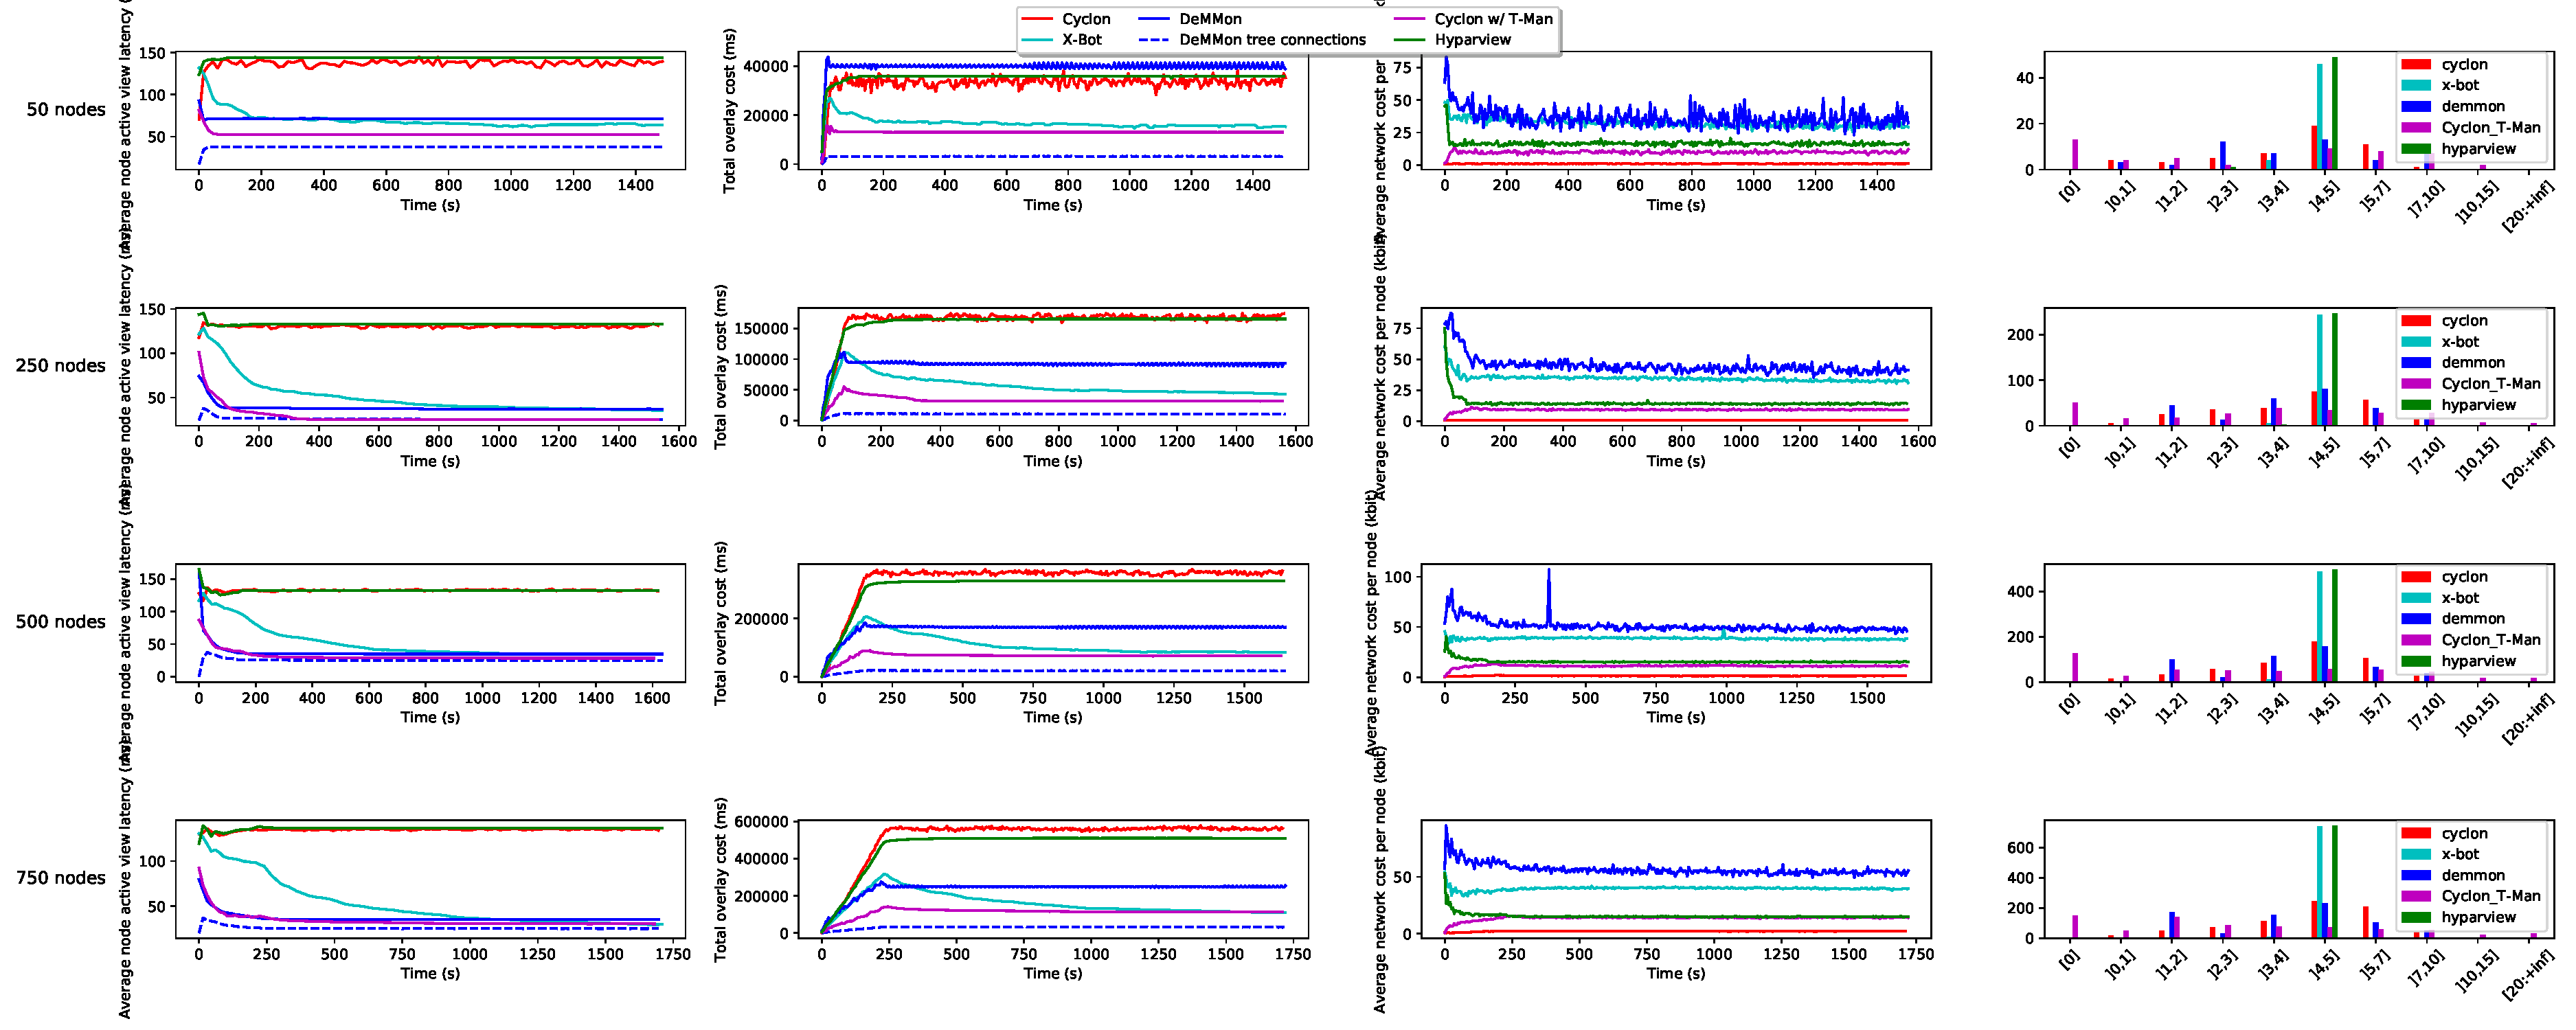
\includegraphics[width=\linewidth]{Chapters/evaluation/figures/membership_0_failures.pdf}
%             \caption{Overlay protocol comparison with failures 0 failures for network sizes of 50, 250, 500 and 750 nodes.}
%             \label{fig:overlay_proto_res_net_building:0_failures}
%         \end{figure}
%     \end{landscape}
% \restoregeometry

% \newgeometry{margin=1cm}
%     \begin{landscape}
%         \thispagestyle{empty}
%         \begin{figure}
%             \centering
%             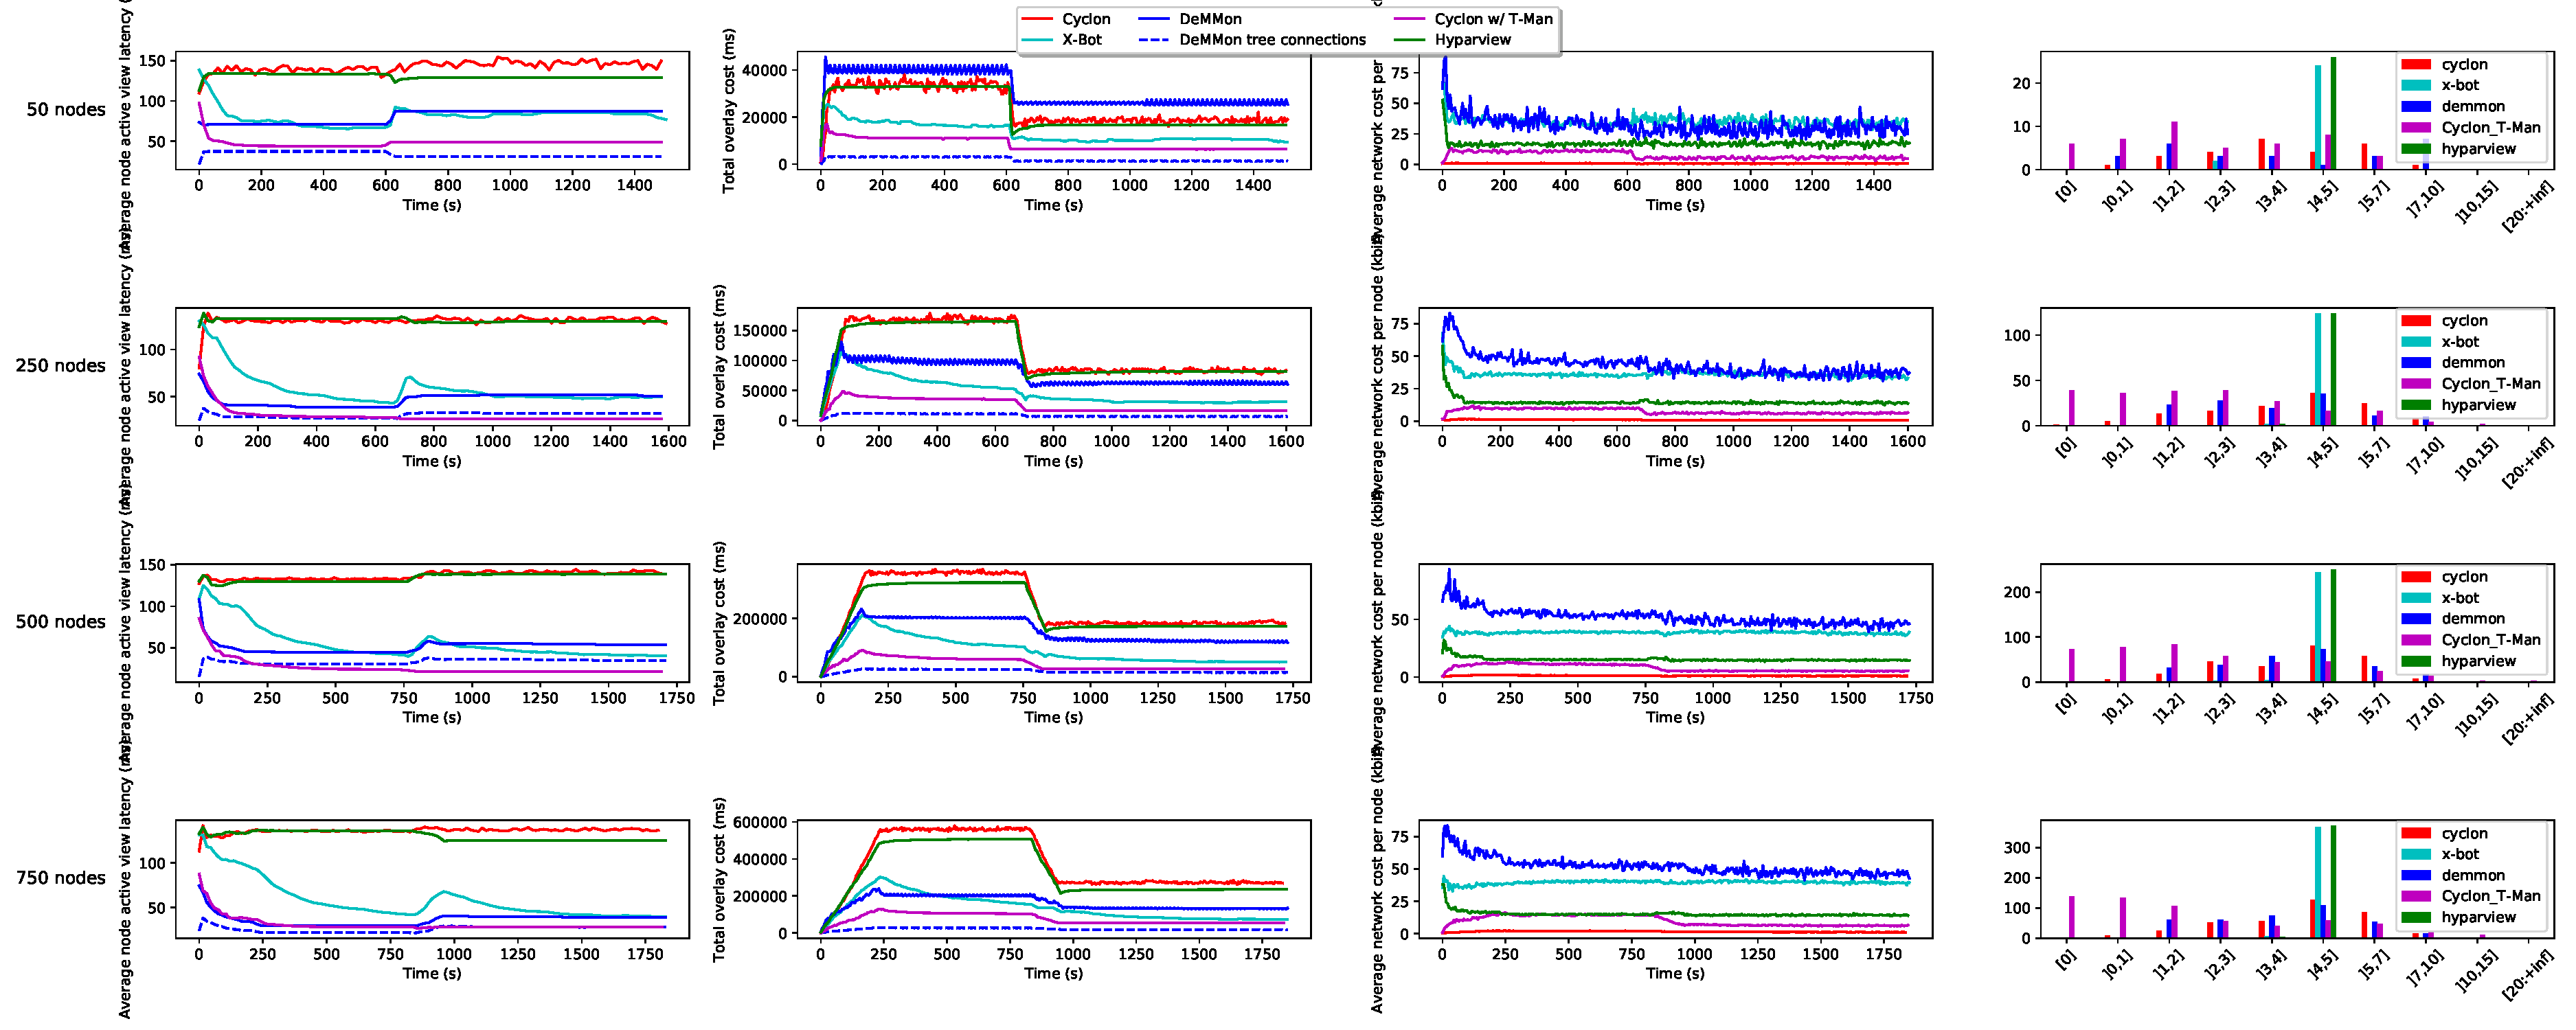
\includegraphics[width=\linewidth]{Chapters/evaluation/figures/membership_50_failures.pdf}
%             \caption{Overlay protocol comparison with failures 50\% failures for network sizes of 50, 250, 500 and 750 nodes.}
%             \label{ig:overlay_proto_res_net_building:50_failures}
%         \end{figure}
%     \end{landscape}
% \restoregeometry
